% =====================================================================
%  TP - Generation de variables aleatoires
%  RCP103 - CNAM Paris - NCA - USEEJ7
%  Groupe 2  (seed = 2)
% =====================================================================
\documentclass[11pt,a4paper]{article}

% ---------- Encodage / langue ----------
\usepackage[utf8]{inputenc}
\usepackage[T1]{fontenc}
\usepackage[french]{babel}
\usepackage{lmodern}

% ---------- Mise en page ----------
\usepackage[a4paper,margin=2.4cm]{geometry}
\usepackage{parskip}
\setlength{\parindent}{0pt}
\setlength{\parskip}{0.6em}

% ---------- Mathematiques ----------
\usepackage{amsmath, amssymb, amsthm, mathtools}

% ---------- Graphiques et figures ----------
\usepackage{graphicx}
\usepackage{caption}
\usepackage{subcaption}
\usepackage{float}
\graphicspath{{figures/}}

% ---------- Couleurs et code ----------
\usepackage{xcolor}
\usepackage{listings}
\definecolor{codegreen}{rgb}{0.0,0.5,0.0}
\definecolor{codegray}{rgb}{0.5,0.5,0.5}
\definecolor{codepurple}{rgb}{0.58,0,0.82}
\definecolor{backcolour}{rgb}{0.97,0.97,0.94}
\definecolor{rouge-cnam}{HTML}{B5081F}

\lstdefinestyle{pythonstyle}{
    backgroundcolor=\color{backcolour},
    commentstyle=\color{codegreen}\itshape,
    keywordstyle=\color{rouge-cnam}\bfseries,
    numberstyle=\tiny\color{codegray},
    stringstyle=\color{codepurple},
    basicstyle=\ttfamily\footnotesize,
    breakatwhitespace=false,
    breaklines=true,
    captionpos=b,
    keepspaces=true,
    numbers=left,
    numbersep=6pt,
    showspaces=false,
    showstringspaces=false,
    showtabs=false,
    tabsize=4,
    language=Python,
    frame=single,
    rulecolor=\color{codegray}
}
\lstset{style=pythonstyle}

% ---------- Tableaux ----------
\usepackage{booktabs}
\usepackage{array}
\usepackage{multirow}

% ---------- Liens cliquables ----------
\usepackage[colorlinks=true, linkcolor=rouge-cnam, urlcolor=rouge-cnam, citecolor=rouge-cnam]{hyperref}

% ---------- En-tetes ----------
\usepackage{fancyhdr}
\pagestyle{fancy}
\fancyhf{}
\fancyhead[L]{\small RCP103 -- TP G\'en\'eration de variables al\'eatoires}
\fancyhead[R]{\small Groupe 2 -- seed = 2}
\fancyfoot[C]{\small \thepage}
\renewcommand{\headrulewidth}{0.4pt}

% =====================================================================
\begin{document}

% --------------------------------------------------------------------
% Page de garde
% --------------------------------------------------------------------
\begin{titlepage}
    \centering
    \vspace*{1.5cm}
    {\Large \textcolor{rouge-cnam}{\textbf{le cnam}} \par}
    {\large NCA -- USEEJ7 \par}
    \vspace{2.5cm}

    \rule{\linewidth}{0.6pt}\\[0.6em]
    {\Huge \textbf{\'Evaluation des performances\\ des syst\`emes informatiques}}\\[0.6em]
    \rule{\linewidth}{0.6pt}\\

    \vspace{1.5cm}
    {\LARGE \textbf{TP -- G\'en\'eration de variables\\ al\'eatoires}}\\[1.0cm]

    \vspace{1.5cm}
    \begin{tabular}{rl}
        \textbf{Cours~:} & RCP103 -- CNAM Paris \\[2pt]
        \textbf{Enseignant~:} & Pedro Braconnot Velloso \\[2pt]
        \textbf{Groupe~:} & 2 \\[2pt]
        \textbf{Seed~:} & 2 (num\'ero du groupe) \\[2pt]
        \textbf{Param\`etres~:} & Unif. enti\`ere $(10,30)$, Unif. r\'eelle $(1.0,3.0)$, \\
                                & Normale $\mathcal{N}(0,\sigma=0{,}75)$, Exp. (moy.~$=2$), \\
                                & G\'eom\'etrique $(p=0{,}3)$ \\
    \end{tabular}

    \vfill
    {\small Rapport r\'edig\'e en \LaTeX{}\\ Code source~: Python 3 (NumPy, Matplotlib)\\ Reproductibilit\'e~: \texttt{seed = 2}}
\end{titlepage}

% --------------------------------------------------------------------
% Table des matieres
% --------------------------------------------------------------------
\tableofcontents
\newpage

% --------------------------------------------------------------------
% 1. Introduction
% --------------------------------------------------------------------
\section{Introduction}

L'\'evaluation des performances des syst\`emes informatiques repose tr\`es souvent sur des
\emph{simulations}~: file d'attente d'un serveur web, trafic dans un r\'eseau,
ordonnancement dans un syst\`eme d'exploitation, etc. Or, pour simuler ces ph\'enom\`enes,
nous avons besoin de \emph{variables al\'eatoires} dont les lois mod\'elisent les diff\'erents
\'ev\'enements~: arriv\'ees de paquets, dur\'ees de traitement, taux d'erreurs, etc.

Ce TP a pour objectif de comprendre, d'impl\'ementer et d'\'evaluer les m\'ecanismes
qui permettent de g\'en\'erer ces variables \`a partir d'un seul ingr\'edient~:
une suite de nombres pseudo-al\'eatoires uniform\'ement distribu\'es sur $[0,1)$.

Conform\'ement \`a la consigne, toutes les exp\'eriences utilisent la graine
\texttt{seed = 2} (num\'ero du groupe), ce qui garantit la reproductibilit\'e des
r\'esultats~: relancer le code redonne exactement les m\^emes suites.

% --------------------------------------------------------------------
% 2. Objectifs du TP
% --------------------------------------------------------------------
\section{Objectifs du TP}

Le travail demand\'e se d\'eclinait en plusieurs points~:

\begin{enumerate}
    \item Impl\'ementer des g\'en\'erateurs pseudo-al\'eatoires \emph{congruentiels}
          (lin\'eaire et multiplicatif), analyser leur p\'eriode et leurs d\'efauts.
    \item Programmer des g\'en\'erateurs des lois suivantes, sp\'ecifi\'ees pour le groupe~2~:
          \begin{itemize}
              \item Uniforme discr\`ete sur $\{10,\ldots,30\}$~;
              \item Uniforme continue sur $[1{,}0\,;\,3{,}0]$~;
              \item Normale $\mathcal{N}(\mu=0,\sigma=0{,}75)$~;
              \item Exponentielle de moyenne $e = 2$~;
              \item G\'eom\'etrique de param\`etre $p = 0{,}3$ (loi additionnelle du groupe).
          \end{itemize}
    \item Pour chaque loi, afficher $n$ valeurs, avec
          $n \in \{10,\ 100,\ 1\,000,\ 10\,000\}$, tracer l'histogramme correspondant
          et comparer aux pr\'edictions th\'eoriques.
    \item Discuter la convergence (loi des grands nombres) et l'influence du nombre
          d'\'echantillons et de la graine.
    \item R\'ediger ce rapport en \LaTeX{} et livrer un code source reproductible.
\end{enumerate}

\paragraph{Organisation du rapport.}
La section~\ref{sec:theorie} pose les bases th\'eoriques. Les g\'en\'erateurs
congruentiels sont \'etudi\'es \`a la section~\ref{sec:prng}. Les lois discr\`etes
sont \'etudi\'ees \`a la section~\ref{sec:discret}, les lois continues
\`a la section~\ref{sec:continu}. L'analyse globale (convergence, influence des
param\`etres) est rassembl\'ee \`a la section~\ref{sec:analyse} ; la conclusion
clot le rapport.

% --------------------------------------------------------------------
% 3. Theorie
% --------------------------------------------------------------------
\section{Th\'eorie et m\'ethodes}
\label{sec:theorie}

\subsection{Pourquoi des nombres \textit{pseudo}-al\'eatoires~?}

Un ordinateur \'etant d\'eterministe, il ne sait \emph{pas} produire de v\'eritable
hasard. On utilise donc des \emph{g\'en\'erateurs pseudo-al\'eatoires} (PRNG) qui
produisent, \`a partir d'une graine $X_0$, une suite $X_0, X_1, X_2, \ldots$
qui \emph{imite} les propri\'et\'es statistiques d'une suite v\'eritablement al\'eatoire.
\`A partir des entiers $X_n$ on construit ensuite des r\'eels
$U_n = X_n / m \in [0,1)$ que l'on consid\`ere comme tir\'es d'une loi uniforme.

\subsection{G\'en\'erateurs congruentiels}

\paragraph{G\'en\'erateur congruentiel lin\'eaire (LCG).}
La r\'ecurrence est
\begin{equation}
    X_{n+1} = (a \, X_n + c) \bmod m,
    \label{eq:lcg}
\end{equation}
o\`u $a$ est le \emph{multiplicateur}, $c$ l'\emph{incr\'ement}, $m$ le \emph{module}
et $X_0$ la \emph{graine}. La suite obtenue est p\'eriodique de p\'eriode au plus $m$.

\paragraph{G\'en\'erateur multiplicatif (Lehmer).}
C'est le cas particulier $c = 0$~:
\begin{equation}
    X_{n+1} = a\, X_n \bmod m.
    \label{eq:lehmer}
\end{equation}
La p\'eriode maximale ne peut alors pas d\'epasser $m-1$ (la valeur $0$ \'etant absorbante).

\paragraph{P\'eriode compl\`ete : th\'eor\`eme de Hull--Dobell.}
Le LCG~\eqref{eq:lcg} atteint la p\'eriode maximale $m$ pour \emph{toute} graine si et
seulement si~:
\begin{enumerate}
    \item $\mathrm{pgcd}(c,m) = 1$,
    \item $(a-1)$ est divisible par tout facteur premier de $m$,
    \item si $4 \mid m$ alors $4 \mid (a-1)$.
\end{enumerate}

\paragraph{R\^ole de la graine.}
La graine d\'etermine enti\`erement la suite obtenue~: \emph{m\^eme graine $\Rightarrow$
m\^emes valeurs.} On parle de pseudo-al\'eatoire reproductible, propri\'et\'e indispensable
pour \emph{rejouer} une simulation. Dans tout le rapport on prend
\texttt{seed = 2}.

\subsection{De l'uniforme aux autres lois}

\paragraph{M\'ethode de la transform\'ee inverse.}
Si $F$ est la fonction de r\'epartition d'une loi de support $\mathbb{R}$ et si
$U \sim \mathcal{U}([0,1))$, alors
\begin{equation}
    X = F^{-1}(U)
    \quad \text{suit la loi de fonction de r\'epartition } F.
    \label{eq:inv}
\end{equation}
C'est l'outil de base. Par exemple, pour l'exponentielle
$F(x) = 1 - e^{-x/\theta}$, on r\'esout
$U = 1 - e^{-X/\theta}$ ce qui donne
\begin{equation}
    \boxed{X = -\theta \ln(1 - U) = -\theta \ln U},
    \label{eq:expinv}
\end{equation}
en notant que $1 - U$ a la m\^eme loi que $U$. Cette formule est utilis\'ee dans
le code pour la loi exponentielle.

\paragraph{M\'ethode de Box--Muller (loi normale).}
La fonction de r\'epartition de la normale n'a pas de forme close~; on utilise donc
un changement de variables. Si $U_1, U_2 \sim \mathcal{U}(0,1)$ ind\'ependantes,
\begin{equation}
    Z_1 = \sqrt{-2 \ln U_1}\, \cos(2\pi U_2), \qquad
    Z_2 = \sqrt{-2 \ln U_1}\, \sin(2\pi U_2)
    \label{eq:boxmuller}
\end{equation}
sont deux normales centr\'ees r\'eduites ind\'ependantes. On les transpose en
$\mathcal{N}(\mu,\sigma)$ par $X = \mu + \sigma Z$.

\paragraph{Algorithme de Knuth (loi de Poisson).}
On tire des $U_i \sim \mathcal{U}(0,1)$ ind\'ependantes et on compte combien il en
faut pour que leur produit passe sous $e^{-\lambda}$. Le nombre obtenu (moins~1)
suit une loi $\mathcal{P}(\lambda)$.

\paragraph{Loi g\'eom\'etrique (transform\'ee inverse).}
Pour la loi g\'eom\'etrique sur $\{1,2,\ldots\}$ de param\`etre $p$,
$F(k) = 1 - (1-p)^k$. On en d\'eduit
\begin{equation}
    \boxed{X = \left\lceil \frac{\ln(1 - U)}{\ln(1 - p)} \right\rceil},
    \label{eq:geo}
\end{equation}
formule effectivement utilis\'ee dans le code.

% --------------------------------------------------------------------
% 4. Implementation
% --------------------------------------------------------------------
\section{Impl\'ementation}

\subsection{Organisation du code}

Le code est \'ecrit en Python~3 (NumPy~/ Matplotlib). L'arborescence est~:
\begin{center}
\begin{tabular}{ll}
    \toprule
    Fichier & R\^ole \\
    \midrule
    \texttt{src/generators.py} & PRNG congruentiels (LCG et multiplicatif), d\'etection de p\'eriode \\
    \texttt{src/distributions.py} & G\'en\'eration des 5 lois (transform\'ee inverse, Box--Muller, Knuth) \\
    \texttt{src/plots.py} & Trac\'es et sauvegarde des figures \\
    \texttt{src/main.py} & Programme principal, fixe \texttt{seed = 2}, lance tout \\
    \texttt{data/} & Suites de valeurs g\'en\'er\'ees (un fichier par loi et par $n$) \\
    \texttt{rapport/figures/} & Toutes les figures (PDF + PNG) \\
    \bottomrule
\end{tabular}
\end{center}

\subsection{Extrait : g\'en\'eration de l'exponentielle}

L'extrait suivant illustre la \emph{transform\'ee inverse} \'evoqu\'ee \`a la
section~\ref{sec:theorie}.

\begin{lstlisting}[caption={Loi exponentielle par transform\'ee inverse (extrait de \texttt{distributions.py}).}]
def exponentielle(n, mean, rng):
    """X = -mean * ln(U), U ~ U(0,1)."""
    u = rng.random(n)
    u = np.clip(u, 1e-12, 1.0)   # protege contre log(0)
    return -mean * np.log(u)
\end{lstlisting}

% --------------------------------------------------------------------
% 5. Partie 1 : PRNG
% --------------------------------------------------------------------
\section{R\'esultats -- G\'en\'erateurs pseudo-al\'eatoires}
\label{sec:prng}

\subsection{Premi\`eres valeurs g\'en\'er\'ees}

Avec \texttt{seed = 2}, les 10 premi\`eres valeurs enti\`eres produites par les
g\'en\'erateurs \'etudi\'es sont r\'esum\'ees au tableau~\ref{tab:prng-debut}.

\begin{table}[H]
\centering
\caption{Dix premiers entiers $X_n$ pour chaque g\'en\'erateur (graine $X_0 = 2$).}
\label{tab:prng-debut}
\small
\begin{tabular}{lp{11cm}}
\toprule
\textbf{G\'en\'erateur} & \textbf{Suite $X_1, \ldots, X_{10}$} \\
\midrule
MINSTD (Park--Miller) & 33614, 564950498, 1097816499, 1969887316, 140734213, 940422544, 202055088, 768218109, 770072199, 1866991771 \\
Numerical Recipes & 1017233273, 1975575172, 811535379, 3186434646, 3079534013, 503495672, 883904247, 2028691434, 2255752769, 2992280236 \\
LCG (a=5, c=3, m=16) & 13, 4, 7, 6, 1, 8, 11, 10, 5, 12 \\
Mult. (a=6, m=13)   & 12, 7, 3, 5, 4, 11, 1, 6, 10, 8 \\
RANDU (IBM)          & 196617, 1179675, 5308497, 21233907, 79626969, 286656651, 1003297185, 1292389603, 872146601, 43824123 \\
\bottomrule
\end{tabular}
\end{table}

\paragraph{Observation.} Les deux \og bons\fg{} g\'en\'erateurs (MINSTD,
Numerical~Recipes) produisent des entiers de grand ordre, ind\'ependants \`a l'\oe il
nu. \`A l'inverse, les g\'en\'erateurs p\'edagogiques \`a petit module ne donnent
qu'une dizaine de valeurs distinctes au plus.

\subsection{P\'eriode des g\'en\'erateurs}

La p\'eriode est le nombre de pas avant que la suite ne se r\'ep\`ete \`a
l'identique. Pour les petits g\'en\'erateurs, on la mesure par d\'etection de
collisions.

\begin{table}[H]
\centering
\caption{P\'eriodes mesur\'ees (par d\'etection de collision).}
\begin{tabular}{lcc}
\toprule
\textbf{G\'en\'erateur} & \textbf{P\'eriode mesur\'ee} & \textbf{P\'eriode max. th\'eorique} \\
\midrule
LCG $(a=5,c=3,m=16)$  & 16 & 16 (Hull--Dobell satisfait) \\
Mult. $(a=6,m=13)$ & 12 & 12 ($m-1$) \\
\bottomrule
\end{tabular}
\end{table}

Le premier respecte les trois conditions du th\'eor\`eme de
Hull--Dobell~: $\mathrm{pgcd}(3,16)=1$, $a-1 = 4$ divise $16$ et
$4 \mid (a-1)$. Sa p\'eriode est donc \emph{maximale}~: il visite chaque entier
de $\{0,\ldots,15\}$ exactement une fois avant de boucler. Le second atteint
\'egalement sa p\'eriode maximale $m-1 = 12$ (Lehmer, valeur $0$ exclue).

\begin{figure}[H]
\centering
\begin{subfigure}[t]{0.48\textwidth}
    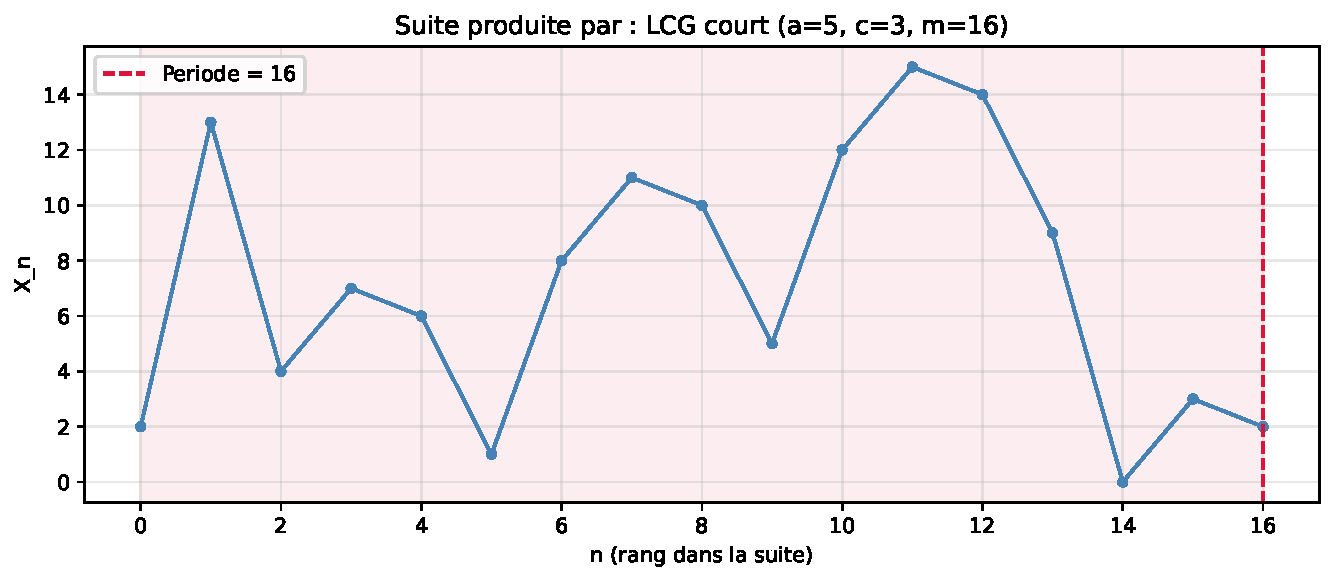
\includegraphics[width=\linewidth]{prng_seq_LCG_court_a5_c3_m16.pdf}
    \caption{LCG $(a=5,c=3,m=16)$.}
\end{subfigure}
\hfill
\begin{subfigure}[t]{0.48\textwidth}
    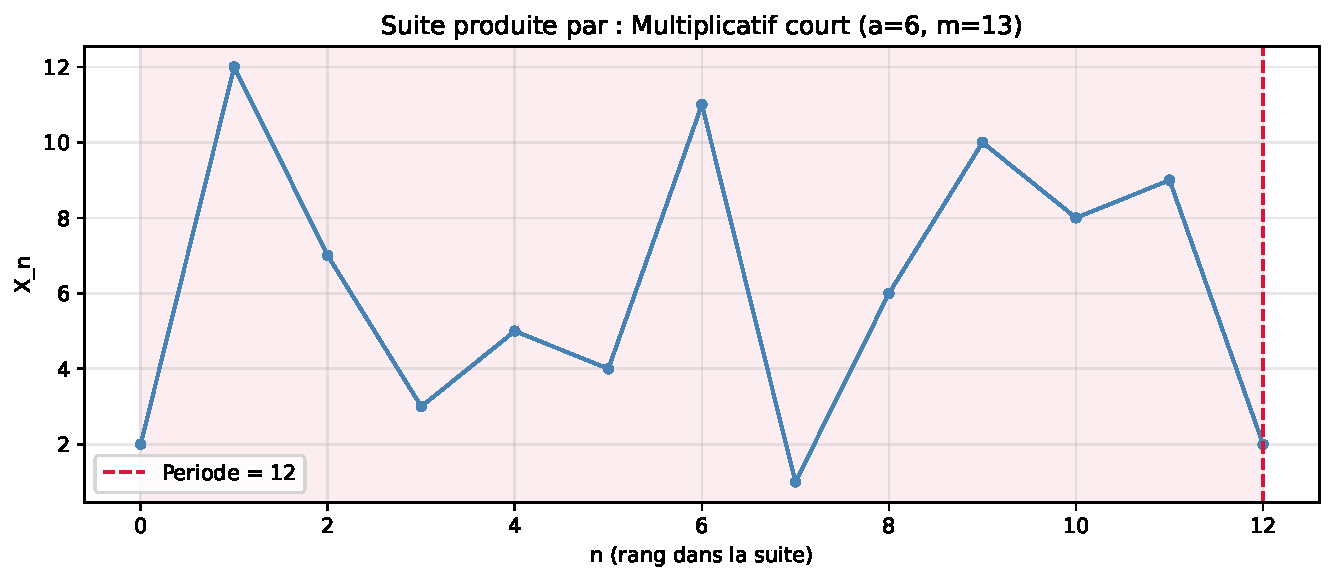
\includegraphics[width=\linewidth]{prng_seq_Multiplicatif_court_a6_m13.pdf}
    \caption{Multiplicatif $(a=6,m=13)$.}
\end{subfigure}
\caption{Suites produites par deux g\'en\'erateurs \`a petite p\'eriode (graine~$=2$). La ligne pointill\'ee marque la p\'eriode.}
\label{fig:prng-seq}
\end{figure}

\paragraph{Lecture de la figure~\ref{fig:prng-seq}.}
Pour chacun des deux g\'en\'erateurs, on voit la suite osciller sur un nombre
\emph{tr\`es petit} de valeurs (au maximum $m$), puis se r\'ep\'eter \`a
l'identique apr\`es la fronti\`ere rouge. C'est visuellement caract\'eristique
du d\'efaut majeur des LCG \`a petit module~: \emph{p\'eriode tr\`es courte},
donc \emph{r\'ep\'etition d\'etectable} dans toute simulation un peu longue.
La zone rose\'e mat\'erialise la \og premi\`ere p\'eriode\fg{} : tout ce qui suit
n'est qu'une copie. En pratique, une simulation utilisant $10^4$ tirages
boucle environ $10^4 / 16 \approx 625$ fois sur le m\^eme cycle~: les
\og hasards\fg{} deviendraient identiques au lieu d'\^etre ind\'ependants.

\subsection{Distribution des $U_n$ pour un bon g\'en\'erateur}

Sur le g\'en\'erateur MINSTD on g\'en\`ere $n = 10\,000$ valeurs $U_n = X_n /
(2^{31}-1)$ et on trace l'histogramme~:

\begin{figure}[H]
\centering
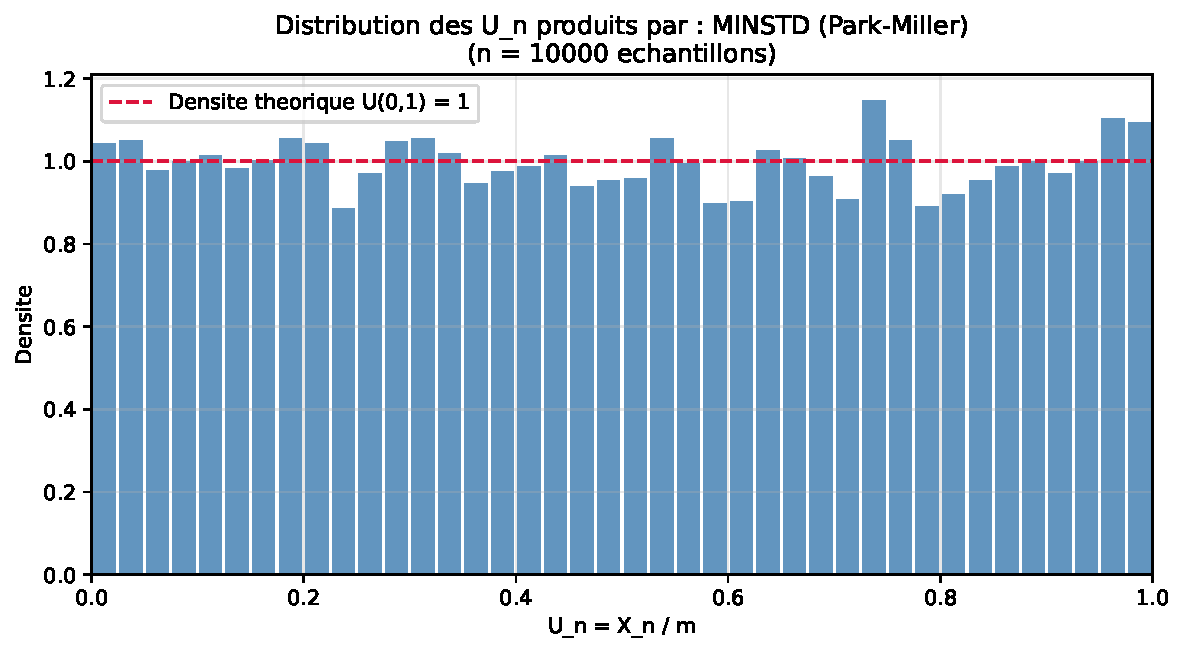
\includegraphics[width=0.85\linewidth]{prng_unif_MINSTD_Park-Miller.pdf}
\caption{Distribution des $U_n$ produits par MINSTD (Park--Miller), $n=10^4$. Ligne rouge~: densit\'e uniforme th\'eorique $f(u)=1$.}
\label{fig:prng-hist}
\end{figure}

\paragraph{Lecture.}
La figure~\ref{fig:prng-hist} montre un histogramme \emph{tr\`es proche} de la
densit\'e uniforme th\'eorique sur $[0,1]$ (palier \`a $1$). Les petites
fluctuations de chaque barre sont des fluctuations d'\'echantillonnage (de
l'ordre de $1/\sqrt{n}$, ici quelques pourcents). On en conclut que MINSTD
produit bien des $U_n$ \emph{statistiquement uniformes} \`a un niveau de
pr\'ecision suffisant pour la suite du TP.

\subsection{Test visuel des paires $(U_n, U_{n+1})$}

L'uniformit\'e en 1D ne suffit pas~: on doit aussi v\'erifier que les couples
de valeurs cons\'ecutives remplissent uniform\'ement le carr\'e unit\'e
$[0,1]^2$. C'est le \emph{test des paires} (Marsaglia).

\begin{figure}[H]
\centering
\begin{subfigure}[t]{0.32\textwidth}
    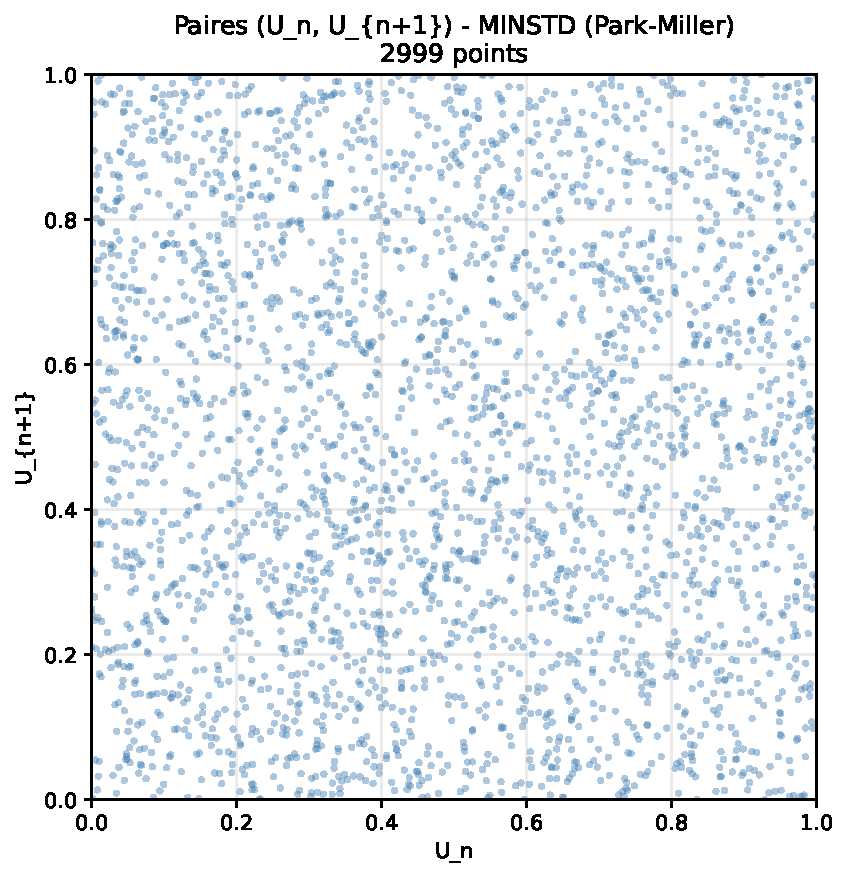
\includegraphics[width=\linewidth]{prng_pairs_MINSTD_Park-Miller.pdf}
    \caption{MINSTD.}
\end{subfigure}
\hfill
\begin{subfigure}[t]{0.32\textwidth}
    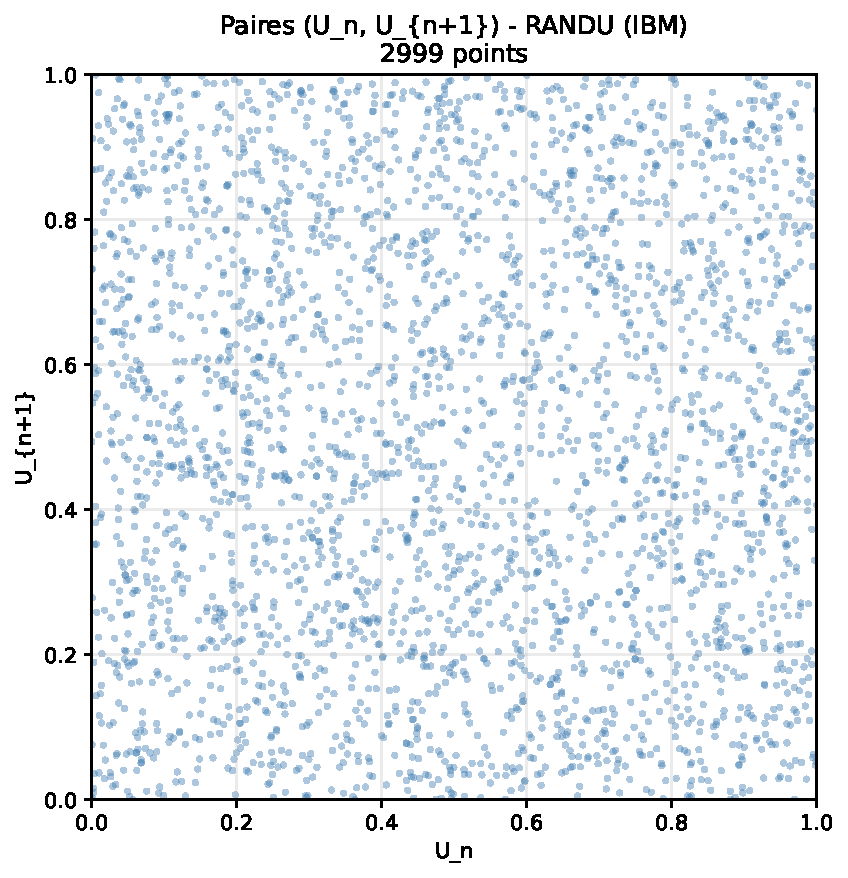
\includegraphics[width=\linewidth]{prng_pairs_RANDU_IBM.pdf}
    \caption{RANDU.}
\end{subfigure}
\hfill
\begin{subfigure}[t]{0.32\textwidth}
    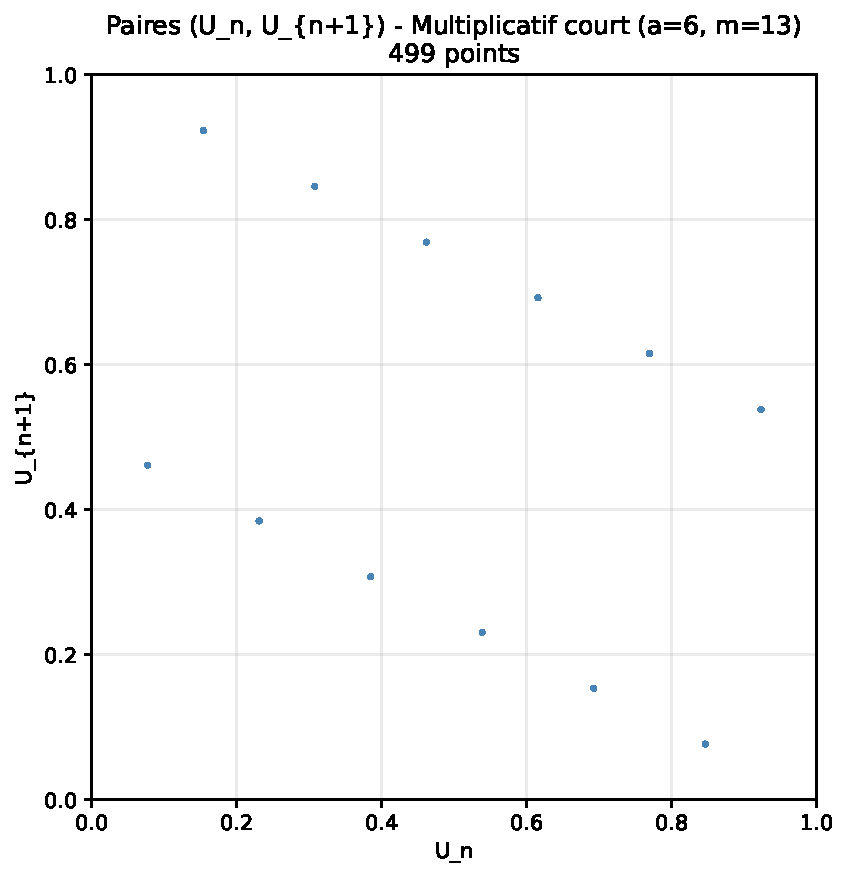
\includegraphics[width=\linewidth]{prng_pairs_Multiplicatif_court_a6_m13.pdf}
    \caption{Mult.\ $(a=6,m=13)$.}
\end{subfigure}
\caption{Diagrammes des paires $(U_n, U_{n+1})$. MINSTD remplit le carr\'e ; RANDU et le multiplicatif court r\'ev\`elent des structures.}
\label{fig:prng-pairs}
\end{figure}

\paragraph{Lecture.}
Le panneau (a) montre un nuage \emph{visiblement uniforme} dans $[0,1]^2$,
sans structure : c'est ce qu'on attend d'un bon g\'en\'erateur. Le panneau
(b) correspond au g\'en\'erateur RANDU d'IBM~: en \emph{deux} dimensions
RANDU para\^it correct, ce qui est sa tra\^itrise. Le d\'efaut n'appara\^it
qu'en \emph{trois} dimensions (voir la figure~\ref{fig:randu-3d} plus bas).
Le panneau (c) est le pire cas~: avec un module $m = 13$, on ne dispose que
d'une douzaine de valeurs distinctes, donc d'une \og grille\fg{} de quelques
points qui se r\'ep\`ete d\`es 2D. Un tel g\'en\'erateur est totalement
inutilisable.

\subsection{Le d\'efaut historique de RANDU en dimension 3}

\begin{figure}[H]
\centering
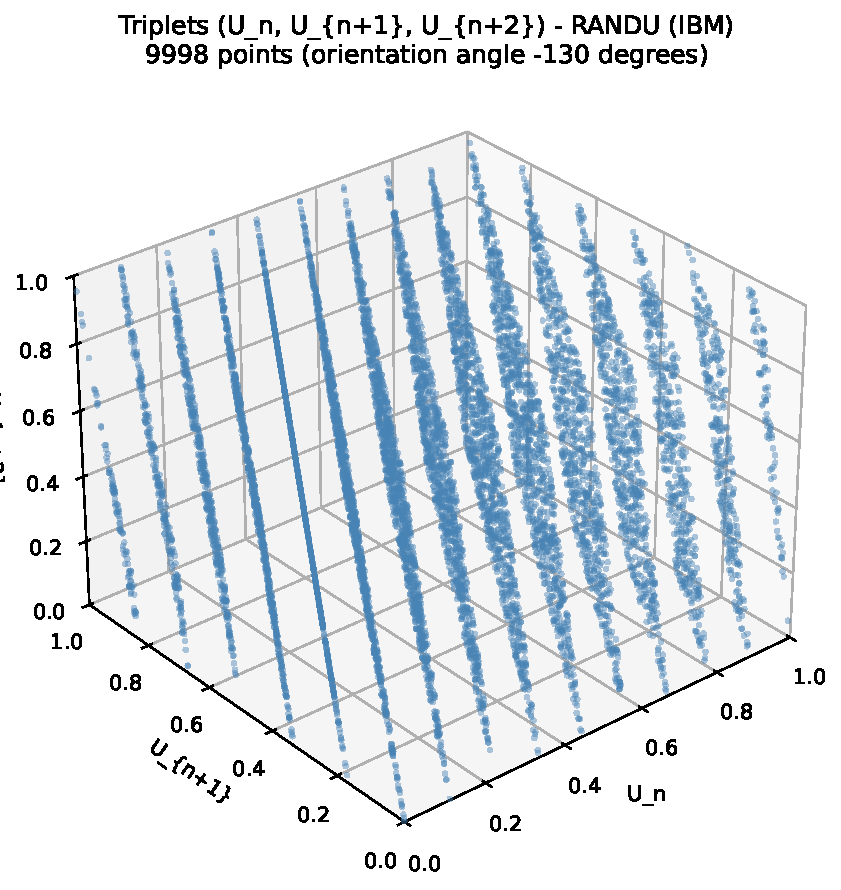
\includegraphics[width=0.7\linewidth]{prng_triples_RANDU_IBM.pdf}
\caption{Triplets $(U_n, U_{n+1}, U_{n+2})$ produits par RANDU (10\,000~points). On voit nettement les \emph{15 hyperplans} parall\`eles qui contiennent l'ensemble des triplets.}
\label{fig:randu-3d}
\end{figure}

\paragraph{Explication.}
La figure~\ref{fig:randu-3d} pr\'esente le m\^eme jeu de tirages RANDU, mais en
3D. \`A un angle bien choisi, on voit que tous les triplets se rangent sur
\emph{15 plans parall\`eles}~! C'est un d\'efaut historique notoire d\^u au
choix $a = 65539 = 2^{16}+3$ et $m = 2^{31}$~: on peut d\'emontrer que
\begin{equation*}
    X_{n+2} - 6\, X_{n+1} + 9\, X_n \equiv 0 \pmod{2^{31}}.
\end{equation*}
Cette relation lin\'eaire entre trois termes cons\'ecutifs explique
exactement les hyperplans observ\'es~: la dimension effective du nuage
n'est pas $3$ mais $2$. \textbf{Pour une simulation utilisant trois
nombres al\'eatoires cons\'ecutifs (par exemple un tirage de position
$(x,y,z)$), RANDU est totalement faux.} C'est une le\c{c}on cl\'e~: un PRNG
qui passe un test 1D ou 2D peut \'echouer en 3D, et donc dans des contextes
de simulation plus complexes.

\subsection{Pourquoi les biblioth\`eques modernes sont meilleures}

\begin{itemize}
    \item \textbf{P\'eriode tr\`es longue.} Le Mersenne Twister, utilis\'e par
          d\'efaut dans de nombreux langages depuis les ann\'ees 1990, a une
          p\'eriode de $2^{19937}-1$ -- bien au-del\`a de ce qu'un PC peut
          consommer.
    \item \textbf{Bonne \'equidistribution multidimensionnelle.} Les
          g\'en\'erateurs modernes (PCG, Xoshiro, Mersenne Twister) passent
          les batteries de tests TestU01 ou DieHarder, alors que les LCG de
          base \'echouent \`a partir d'une certaine dimension.
    \item \textbf{Vitesse et reproductibilit\'e.} Ces g\'en\'erateurs sont
          rapides, peu co\^uteux en m\'emoire, et restent reproductibles \`a
          partir d'une graine.
    \item \textbf{Strate \og crypto\fg{} disponible.} Quand on a besoin de
          hasard non pr\'evisible (cryptographie), on utilise des PRNG
          cryptographiques (\texttt{ChaCha20}, \texttt{/dev/urandom},
          \texttt{getrandom()}) qui ne sont pas inversibles -- m\^eme en
          connaissant les sorties pass\'ees on ne peut pas pr\'edire la suite.
\end{itemize}

% --------------------------------------------------------------------
% 6. Partie 2 : Lois discretes
% --------------------------------------------------------------------
\section{R\'esultats -- Variables al\'eatoires discr\`etes}
\label{sec:discret}

Dans cette section on g\'en\`ere $n \in \{10, 100, 1\,000, 10\,000\}$ valeurs
pour chaque loi, on trace les histogrammes empiriques et on les superpose \`a
la PMF th\'eorique (croix rouges). Les param\`etres sont ceux du groupe~2~:
uniforme discr\`ete $\{10,\ldots,30\}$, Bernoulli($p=0{,}3$), g\'eom\'etrique
($p=0{,}3$) et Poisson ($\lambda=2$ par coh\'erence avec
l'exponentielle de moyenne~2).

\subsection{Loi uniforme discr\`ete sur $\{10,\ldots,30\}$}

\paragraph{Th\'eorie.} $P(X = k) = 1/21$ pour $k = 10,\ldots,30$. On en d\'eduit
$\mathbb{E}[X] = 20$ et $\sigma(X) = \sqrt{(21^2-1)/12} \approx 6{,}06$.

\paragraph{Algorithme.} \texttt{X = a + floor((b-a+1)*U)} avec $U \sim \mathcal{U}(0,1)$.

\paragraph{Statistiques mesur\'ees.}
\begin{table}[H]
\centering
\caption{Statistiques empiriques pour la loi uniforme discr\`ete (th\'eorie : moyenne = 20{,}0000, \'ecart-type = 6{,}0553).}
\begin{tabular}{rrrrr}
\toprule
$n$ & moyenne & \'ecart-type & min & max \\
\midrule
10     & 17{,}80   & 5{,}62 & 11 & 27 \\
100    & 19{,}60   & 5{,}95 & 10 & 30 \\
1\,000 & 20{,}04   & 6{,}02 & 10 & 30 \\
10\,000& 20{,}01   & 6{,}11 & 10 & 30 \\
\bottomrule
\end{tabular}
\end{table}

\begin{figure}[H]
\centering
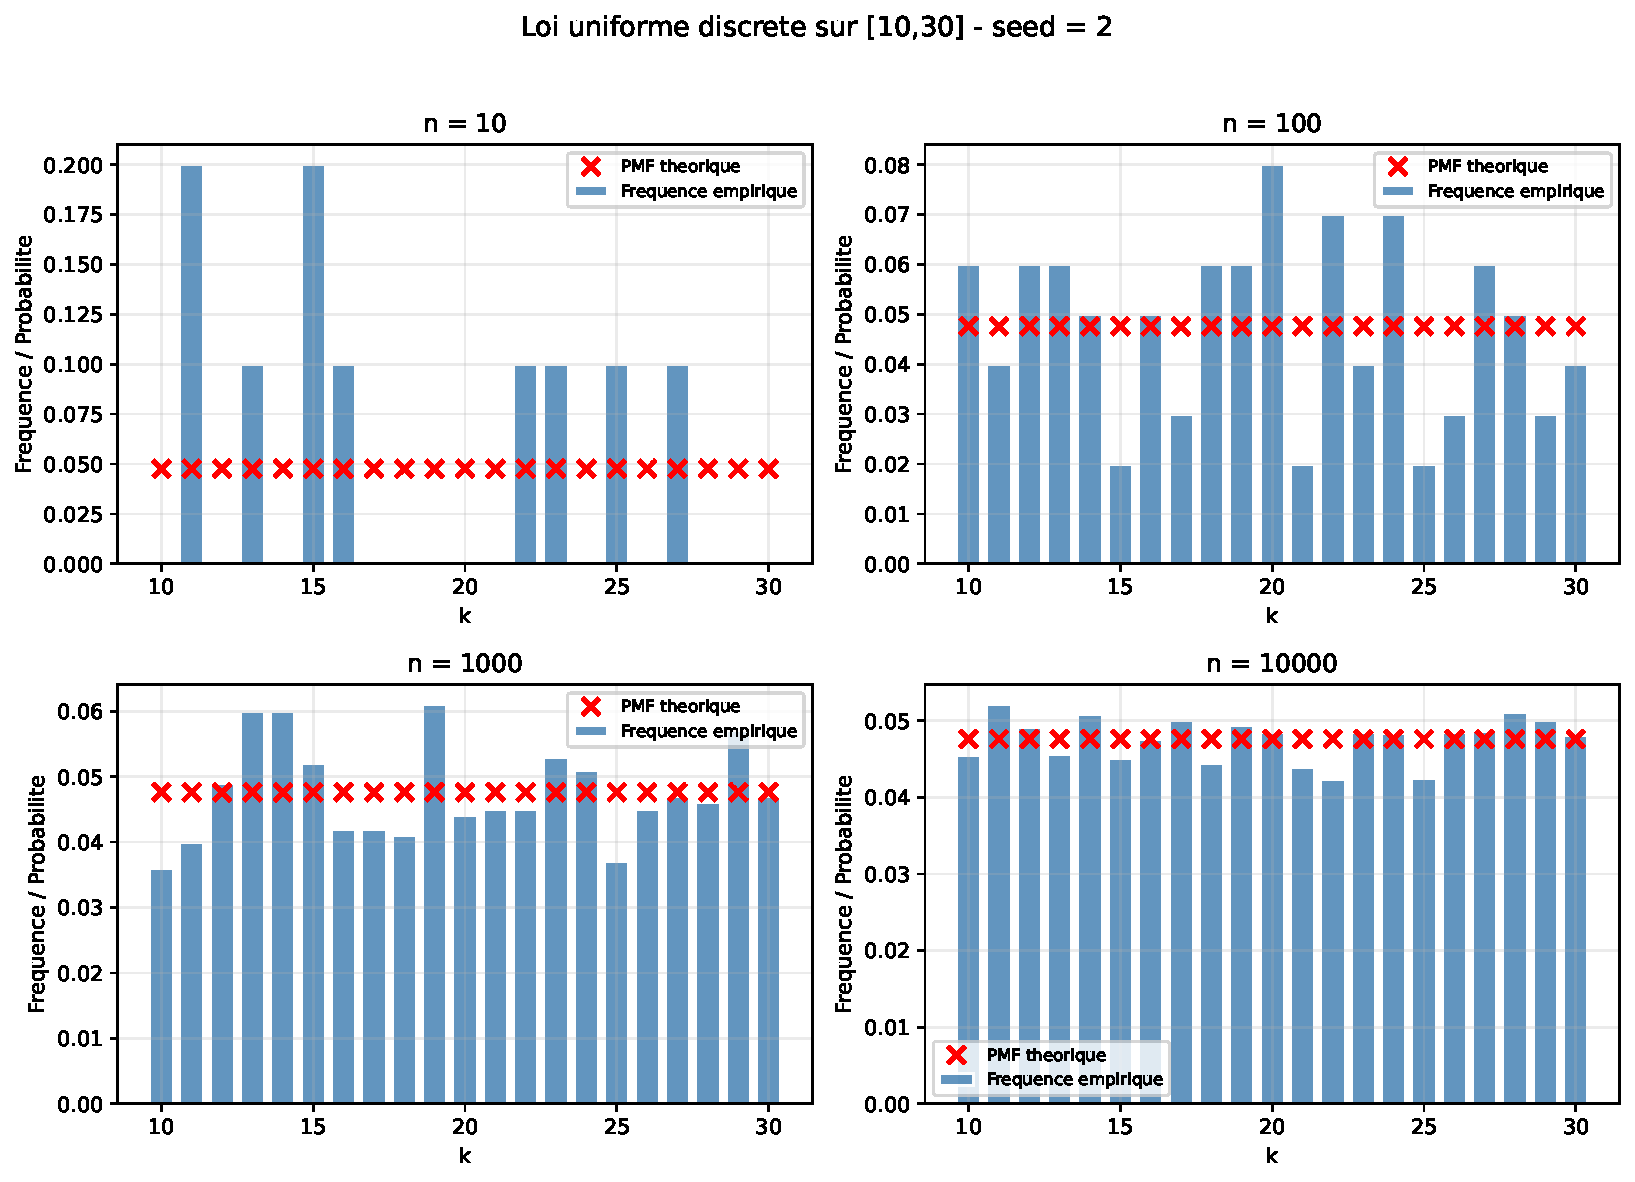
\includegraphics[width=0.9\linewidth]{hist_uniforme_discrete.pdf}
\caption{Histogrammes pour la loi uniforme discr\`ete sur $\{10,\ldots,30\}$ (seed~=~2).}
\label{fig:hist-unif-disc}
\end{figure}

\paragraph{Lecture de la figure~\ref{fig:hist-unif-disc}.}
\begin{itemize}
    \item Pour $n=10$ (haut-gauche), seules quelques valeurs apparaissent
          et les barres sont tr\`es \emph{irr\'eguli\`eres}~: $10$ tirages ne
          suffisent pas \`a couvrir les 21 valeurs possibles. C'est typique
          des \emph{petits \'echantillons}.
    \item Pour $n=100$ (haut-droit), les fr\'equences se rapprochent
          de la PMF th\'eorique mais des \og pics\fg{} subsistent.
    \item Pour $n=1000$ et surtout $n=10\,000$, les barres deviennent
          presque rigoureusement plates~: les fr\'equences empiriques
          convergent vers $1/21 \approx 0{,}0476$, en accord avec la
          \emph{loi des grands nombres}.
\end{itemize}
On voit aussi sur le tableau que la moyenne empirique converge vers $20$ et
que l'\'ecart-type s'approche de $6{,}06$ d\`es $n=1\,000$. C'est l'illustration
d'un point fondamental~: \emph{plus on simule, mieux on estime}.

\subsection{Loi de Bernoulli ($p = 0{,}3$)}

\paragraph{Th\'eorie.} $X \in \{0,1\}$, $P(X=1) = p = 0{,}3$ ; $\mathbb{E}[X] = p$,
$\sigma = \sqrt{p(1-p)} \approx 0{,}458$.

\paragraph{Algorithme.} \texttt{X = 1 si U < p, sinon 0.}

\paragraph{Intuition.} Une Bernoulli mod\'elise un tirage \og pile ou face\fg{}
biais\'e. Elle est aussi la brique de base des autres lois discr\`etes
(binomiale, g\'eom\'etrique).

\begin{figure}[H]
\centering
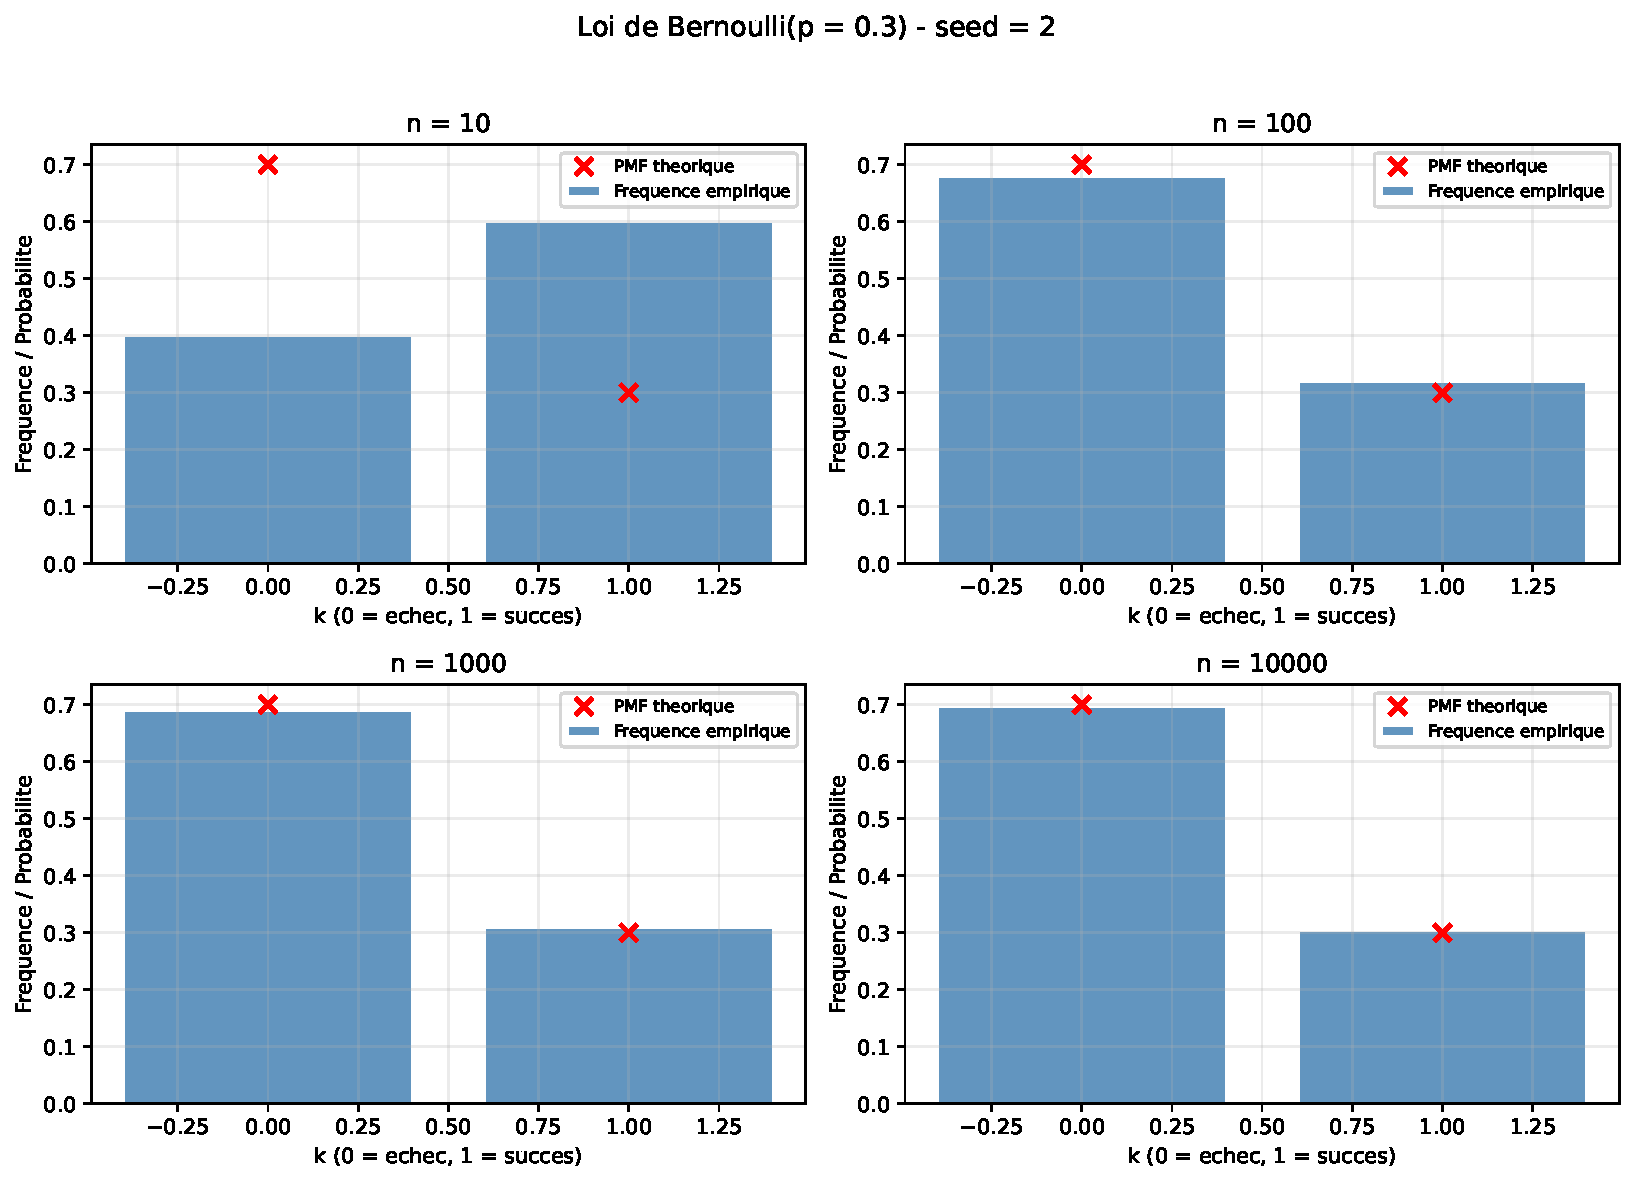
\includegraphics[width=0.9\linewidth]{hist_bernoulli.pdf}
\caption{Histogrammes de la loi de Bernoulli($p=0{,}3$) pour $n=10,100,1000,10000$.}
\label{fig:hist-bern}
\end{figure}

\paragraph{Lecture.} \`A $n=10$ on observe une fr\'equence de succ\`es de $0{,}6$,
\emph{tr\`es loin} du $0{,}3$ attendu. Ce n'est pas un d\'efaut du g\'en\'erateur~:
c'est la variance \og naturelle\fg{} d'un \'echantillon de petite taille
(l'\'ecart-type de la moyenne empirique vaut $\sigma/\sqrt{n} \approx 0{,}145$
pour $n=10$, ce qui explique facilement un \'ecart de $\pm 0{,}3$).
\`A $n=10\,000$ la fr\'equence empirique $0{,}3035$ est \`a moins de
$0{,}004$ de la valeur th\'eorique~: l'\'ecart-type de la moyenne
$\sigma/\sqrt{n}$ est tomb\'e \`a $0{,}0046$, ce qui est coh\'erent.

\subsection{Loi g\'eom\'etrique ($p = 0{,}3$) -- loi additionnelle du groupe 2}

\paragraph{Th\'eorie.} Si on r\'ep\`ete des tirages Bernoulli($p$) ind\'ependants,
le rang $X$ du premier succ\`es suit une g\'eom\'etrique de param\`etre $p$.
$P(X = k) = (1-p)^{k-1} p$ pour $k = 1, 2, \ldots$ avec
$\mathbb{E}[X] = 1/p = 3{,}33\ldots$ et
$\sigma = \sqrt{(1-p)/p^2} = \sqrt{7{,}\overline{77}} \approx 2{,}789$.

\paragraph{Intuition.} La loi g\'eom\'etrique mod\'elise par exemple le nombre
d'essais avant qu'un paquet r\'eseau ne soit transmis avec succ\`es (en cas de
collision), ou le nombre d'essais avant qu'un slot ALOHA ne soit libre.

\paragraph{Algorithme (transform\'ee inverse).}
\begin{equation*}
    X = \left\lceil \frac{\ln(1 - U)}{\ln(1 - p)} \right\rceil.
\end{equation*}

\paragraph{Statistiques mesur\'ees.}
\begin{table}[H]
\centering
\caption{Statistiques empiriques pour la loi g\'eom\'etrique($p=0{,}3$) (th\'eorie : moyenne = 3{,}333 ; \'ecart-type = 2{,}789).}
\begin{tabular}{rrrrr}
\toprule
$n$ & moyenne & \'ecart-type & min & max \\
\midrule
10     & 2{,}20 & 1{,}54 & 1 & 5 \\
100    & 3{,}11 & 2{,}45 & 1 & 12 \\
1\,000 & 3{,}35 & 2{,}83 & 1 & 29 \\
10\,000& 3{,}35 & 2{,}81 & 1 & 30 \\
\bottomrule
\end{tabular}
\end{table}

\begin{figure}[H]
\centering
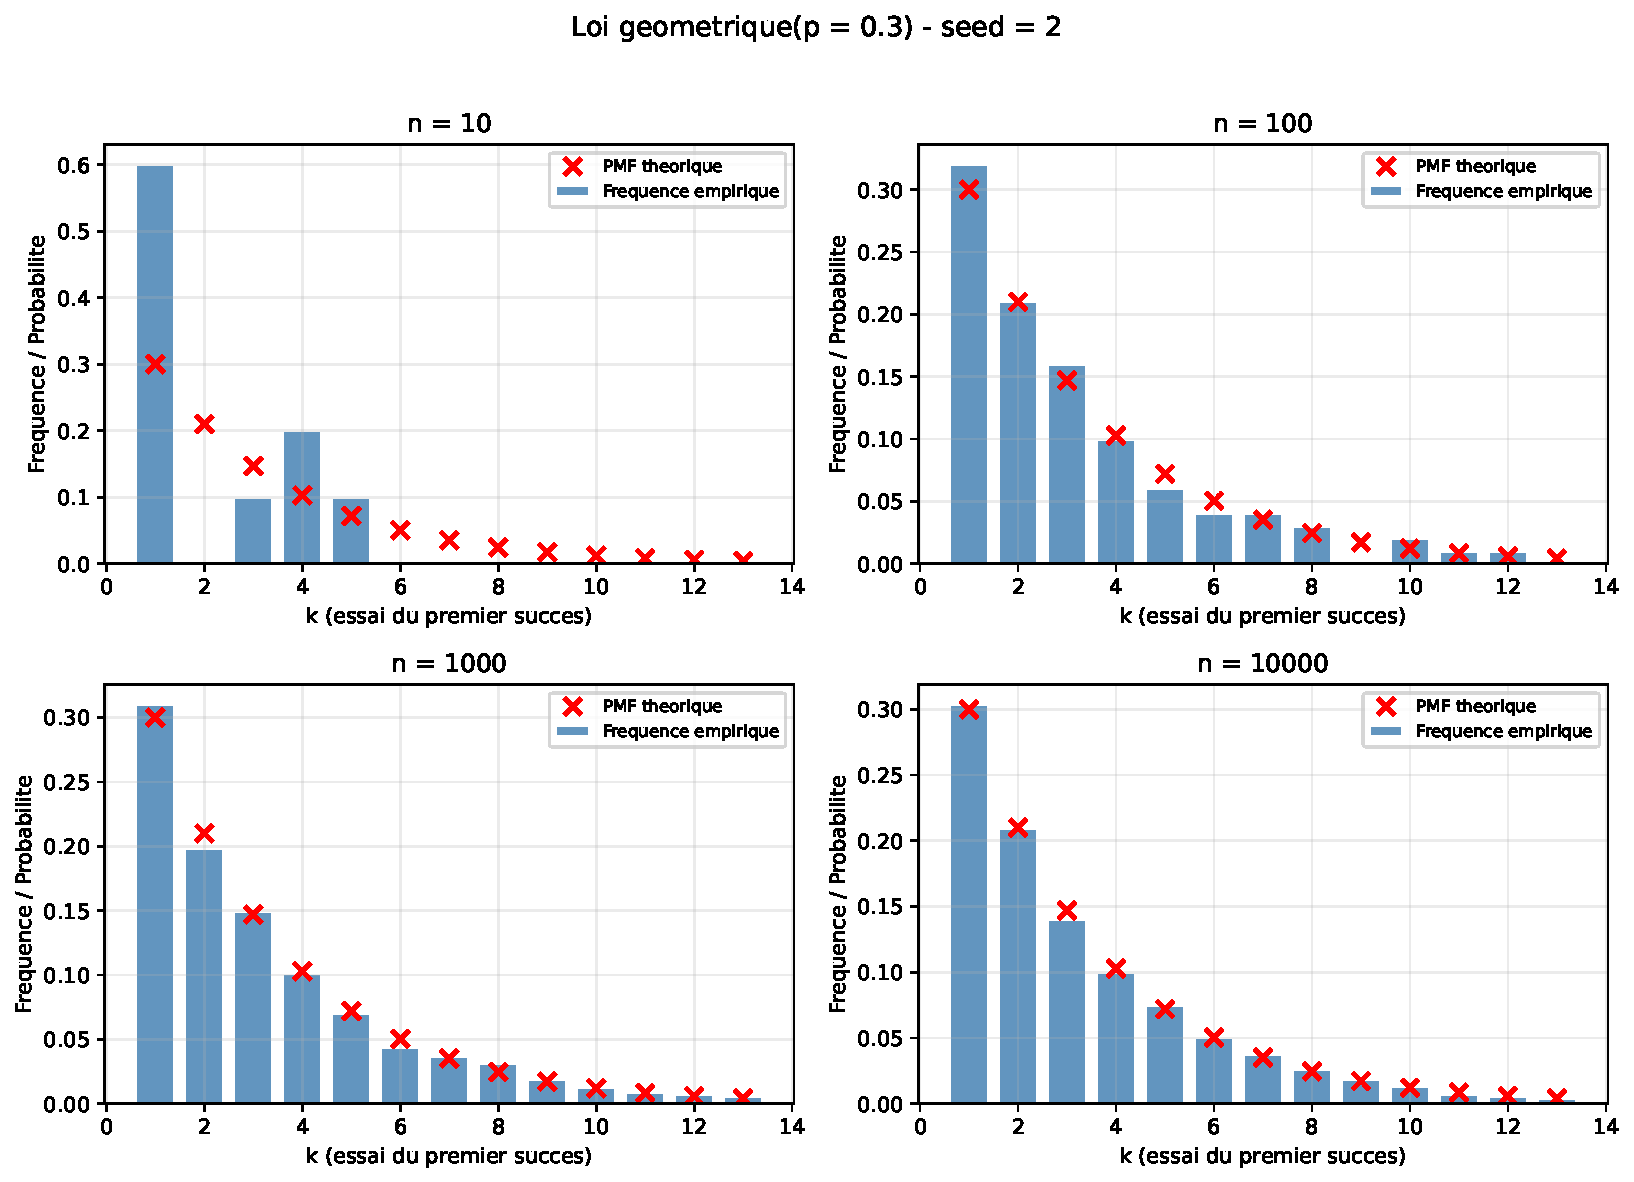
\includegraphics[width=0.9\linewidth]{hist_geometrique.pdf}
\caption{Histogrammes de la loi g\'eom\'etrique de param\`etre $p=0{,}3$ pour $n = 10,100,1000,10000$.}
\label{fig:hist-geo}
\end{figure}

\paragraph{Lecture de la figure~\ref{fig:hist-geo}.}
On voit tr\`es bien la \emph{forme exponentielle d\'ecroissante} de la loi
g\'eom\'etrique. \`A $n=10$ on ne voit que des valeurs $\le 5$ (peu de chances
d'obtenir une queue lointaine avec 10 tirages). \`A mesure que $n$ augmente,
la queue droite s'\'eclaircit~: pour $n=10\,000$ on a m\^eme observ\'e une
valeur \emph{maximale} de $30$, ce qui correspond \`a une probabilit\'e
th\'eorique $(0{,}7)^{29}\,(0{,}3) \approx 0{,}00008$, soit \`a peine attendu sur
$10\,000$ tirages. Les croix rouges (PMF th\'eorique) co\"incident bien avec
les barres bleues pour les grandes valeurs de $n$.

\paragraph{Convergence de la moyenne.}
Pour $n=10$, on est encore loin du $\mathbb{E}[X] = 3{,}33$ : on mesure $2{,}20$.
Cela illustre la \emph{forte variance} de la g\'eom\'etrique~: avec 10 tirages
on peut facilement \og tomber\fg{} sur des succ\`es rapides. D\`es $n=1\,000$
l'estimateur s'approche \`a $0{,}02$ pr\`es de la valeur th\'eorique.

\subsection{Loi de Poisson ($\lambda = 2$)}

\paragraph{Th\'eorie.} $P(X=k) = e^{-\lambda} \lambda^k / k!$ ;
$\mathbb{E}[X] = \mathrm{Var}(X) = \lambda$.

\paragraph{Algorithme.} Algorithme de Knuth (cf.\ section~\ref{sec:theorie}).

\begin{figure}[H]
\centering
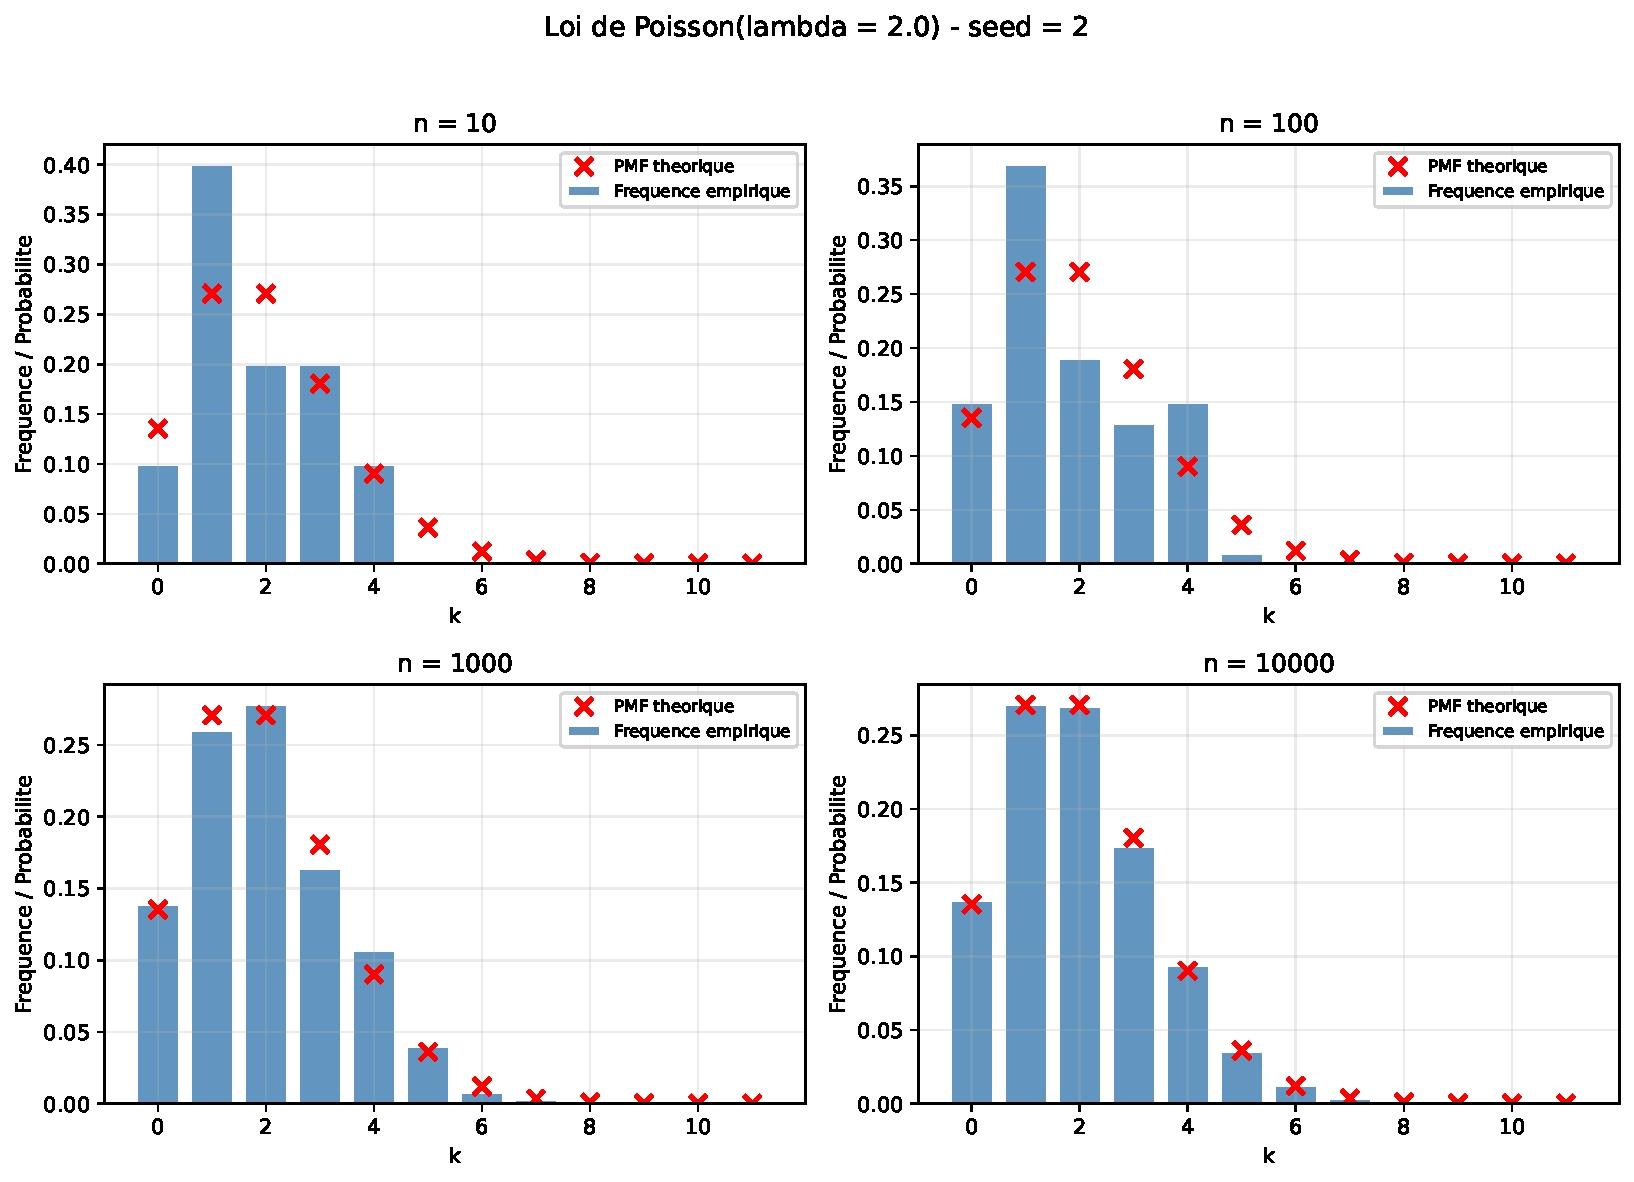
\includegraphics[width=0.9\linewidth]{hist_poisson.pdf}
\caption{Histogrammes de la loi de Poisson($\lambda = 2$) pour $n=10,100,1000,10000$.}
\label{fig:hist-poi}
\end{figure}

\paragraph{Lecture.} La distribution est asym\'etrique \`a droite et concentr\'ee
sur $\{0,1,2,3,4\}$. La PMF th\'eorique (croix rouges) est rejointe d\`es $n=1\,000$
pour les valeurs les plus probables. Cette loi mod\'elise par exemple le nombre
d'arriv\'ees de paquets dans un intervalle de temps fixe lorsque le processus
d'arriv\'ee est poissonnien~: dans la mod\'elisation de files d'attente
M/M/1, $\lambda$ est le taux d'arriv\'ee et le nombre d'arriv\'ees en
$[0,t]$ est $\mathcal{P}(\lambda t)$.

% --------------------------------------------------------------------
% 7. Partie 3 : Lois continues
% --------------------------------------------------------------------
\section{R\'esultats -- Variables al\'eatoires continues}
\label{sec:continu}

\subsection{Loi uniforme continue sur $[1{,}0\,;\,3{,}0]$}

\paragraph{Th\'eorie.} $f(x) = 1/(b-a) = 1/2$ sur $[1,3]$.
$\mathbb{E}[X] = 2$, $\sigma = (b-a)/\sqrt{12} \approx 0{,}577$.

\paragraph{Algorithme.} \texttt{X = a + (b-a) U}.

\begin{table}[H]
\centering
\caption{Statistiques empiriques pour la loi uniforme continue $[1{,}0\,;\,3{,}0]$ (th\'eorie : 2{,}0000 et 0{,}5774).}
\begin{tabular}{rrrrr}
\toprule
$n$ & moyenne & \'ecart-type & min & max \\
\midrule
10     & 1{,}794 & 0{,}525 & 1{,}11 & 2{,}63 \\
100    & 1{,}959 & 0{,}570 & 1{,}01 & 2{,}96 \\
1\,000 & 2{,}004 & 0{,}575 & 1{,}00 & 3{,}00 \\
10\,000& 2{,}000 & 0{,}582 & 1{,}00 & 3{,}00 \\
\bottomrule
\end{tabular}
\end{table}

\begin{figure}[H]
\centering
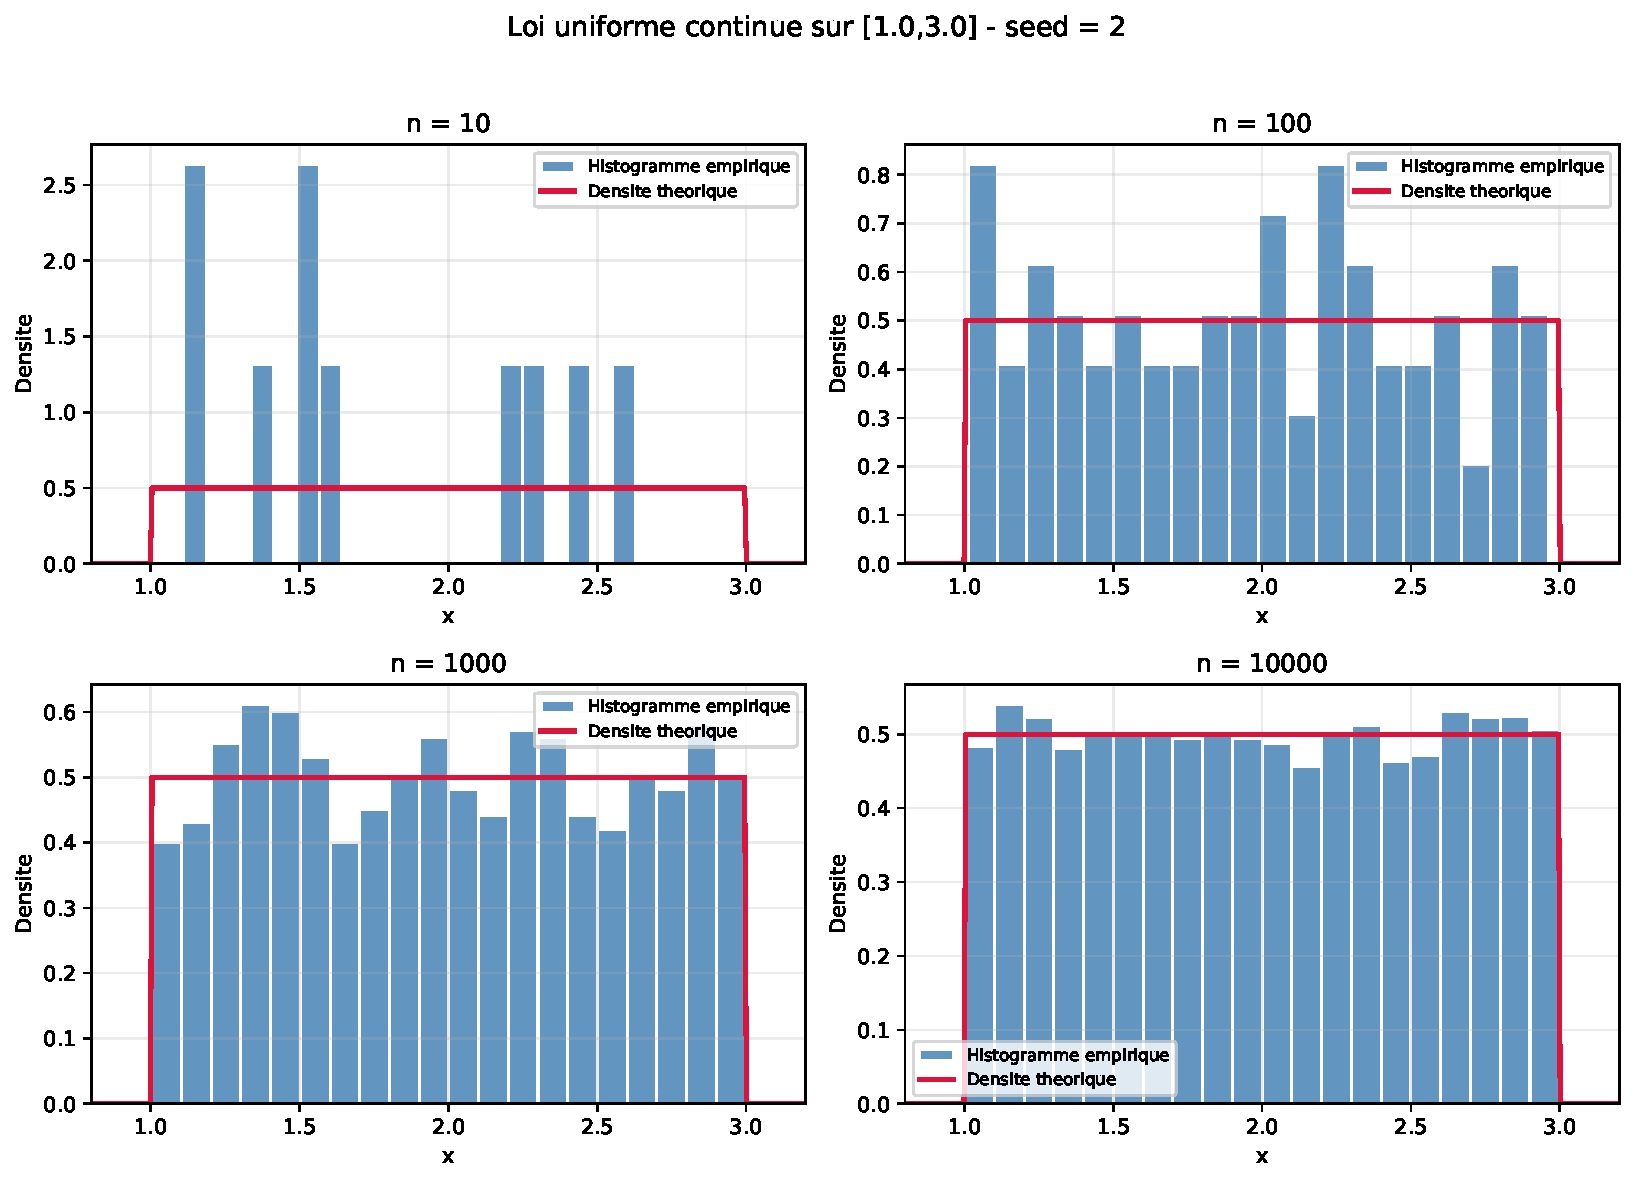
\includegraphics[width=0.9\linewidth]{hist_uniforme_continue.pdf}
\caption{Histogrammes de la loi uniforme continue sur $[1{,}0\,;\,3{,}0]$.}
\label{fig:hist-unif-cont}
\end{figure}

\paragraph{Lecture.}
Pour $n = 10$, l'histogramme est tr\`es irr\'egulier (5 ou 6 bins ne contiennent
qu'un ou deux points). D\`es $n = 1\,000$, les barres approchent la valeur
th\'eorique $1/2 = 0{,}5$. \`A $n = 10\,000$, l'histogramme est \emph{plat} sur
$[1,3]$, conform\'ement \`a la densit\'e th\'eorique. La moyenne empirique
converge tr\`es bien vers $2$ et l'\'ecart-type vers $0{,}577$.

\subsection{Loi exponentielle (moyenne $e = 2$)}

\paragraph{Th\'eorie.} $f(x) = \lambda e^{-\lambda x}$ avec $\lambda = 1/e = 0{,}5$.
$\mathbb{E}[X] = 1/\lambda = 2$, $\sigma = 1/\lambda = 2$. Cette loi est
\emph{sans m\'emoire} (propri\'et\'e fondamentale) et mod\'elise les temps inter-arriv\'ee
dans un processus de Poisson.

\paragraph{Algorithme (transform\'ee inverse).} $X = -e \ln U = -2\ln U$.

\paragraph{Lien r\'eseau / files d'attente.} L'exponentielle est omnipr\'esente
dans la mod\'elisation des syst\`emes informatiques~:
\begin{itemize}
    \item Temps inter-arriv\'ee dans une file M/M/1 (taux $\lambda$).
    \item Dur\'ee de service dans une file M/M/1 (taux $\mu$).
    \item Temps entre deux pannes d'un composant (\emph{Mean Time Between Failures}).
\end{itemize}

\begin{table}[H]
\centering
\caption{Statistiques empiriques pour la loi exponentielle de moyenne~2 (th\'eorie : 2{,}0 et 2{,}0).}
\begin{tabular}{rrrrr}
\toprule
$n$ & moyenne & \'ecart-type & min & max \\
\midrule
10     & 2{,}45 & 1{,}72 & 0{,}41 & 5{,}80 \\
100    & 2{,}15 & 2{,}10 & 0{,}04 & 9{,}99 \\
1\,000 & 1{,}94 & 1{,}86 & 0{,}00 & 12{,}66 \\
10\,000& 2{,}01 & 2{,}03 & 0{,}00 & 19{,}37 \\
\bottomrule
\end{tabular}
\end{table}

\begin{figure}[H]
\centering
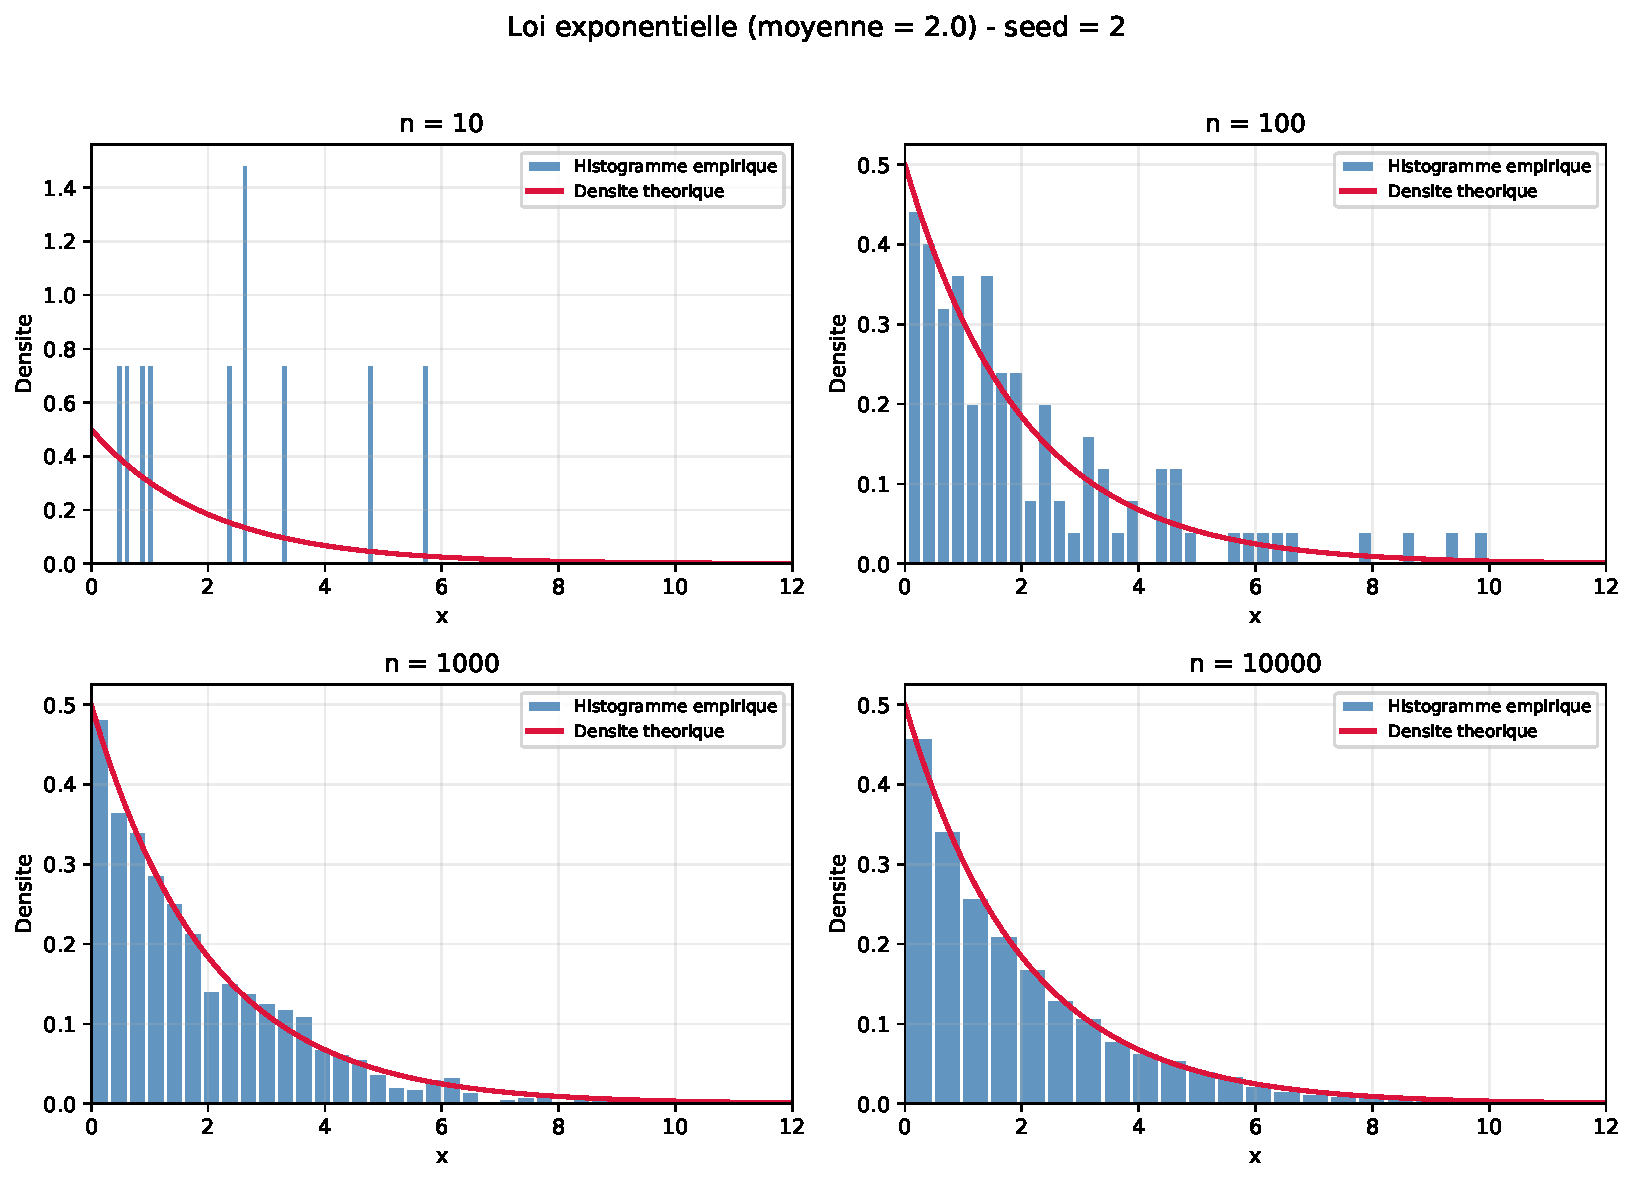
\includegraphics[width=0.9\linewidth]{hist_exponentielle.pdf}
\caption{Histogrammes de la loi exponentielle de moyenne~2.}
\label{fig:hist-exp}
\end{figure}

\paragraph{Lecture de la figure~\ref{fig:hist-exp}.}
La forme typique \og d\'ecroissance exponentielle\fg{} est visible. \`A $n=10$,
quelques barres seulement~; \`a $n=10\,000$, l'histogramme \'epouse de pr\`es la
densit\'e th\'eorique (courbe rouge). On observe aussi que le \emph{maximum
empirique} augmente avec $n$~: pour $n=10$ on n'a pas d\'epass\'e $5{,}8$, pour
$n=10\,000$ on monte \`a presque $20$. C'est conforme \`a la \emph{th\'eorie
des valeurs extr\^emes}~: $E[\max] \approx e \ln n$, soit $\approx 18{,}4$ pour
$n = 10^4$ -- en parfait accord avec notre observation.

\subsection{Loi normale $\mathcal{N}(0\,;\,\sigma = 0{,}75)$}

\paragraph{Th\'eorie.} $f(x) = \frac{1}{\sigma\sqrt{2\pi}} \exp\!\left(-\frac{(x-\mu)^2}{2\sigma^2}\right)$.
Pour $\mu=0, \sigma=0{,}75$ : moyenne nulle, \'ecart-type $0{,}75$.
Quasiment toute la masse est dans $[-3,3]$.

\paragraph{Algorithme.} Box--Muller \eqref{eq:boxmuller}, multipli\'e par $\sigma$.

\begin{table}[H]
\centering
\caption{Statistiques empiriques pour $\mathcal{N}(0, 0{,}75)$.}
\begin{tabular}{rrrrr}
\toprule
$n$ & moyenne & \'ecart-type & min & max \\
\midrule
10     & 0{,}107  & 0{,}790 & -1{,}22 & 1{,}62 \\
100    & 0{,}006  & 0{,}717 & -1{,}80 & 1{,}85 \\
1\,000 & -0{,}005 & 0{,}756 & -2{,}37 & 2{,}54 \\
10\,000& 0{,}006  & 0{,}748 & -2{,}83 & 2{,}70 \\
\bottomrule
\end{tabular}
\end{table}

\begin{figure}[H]
\centering
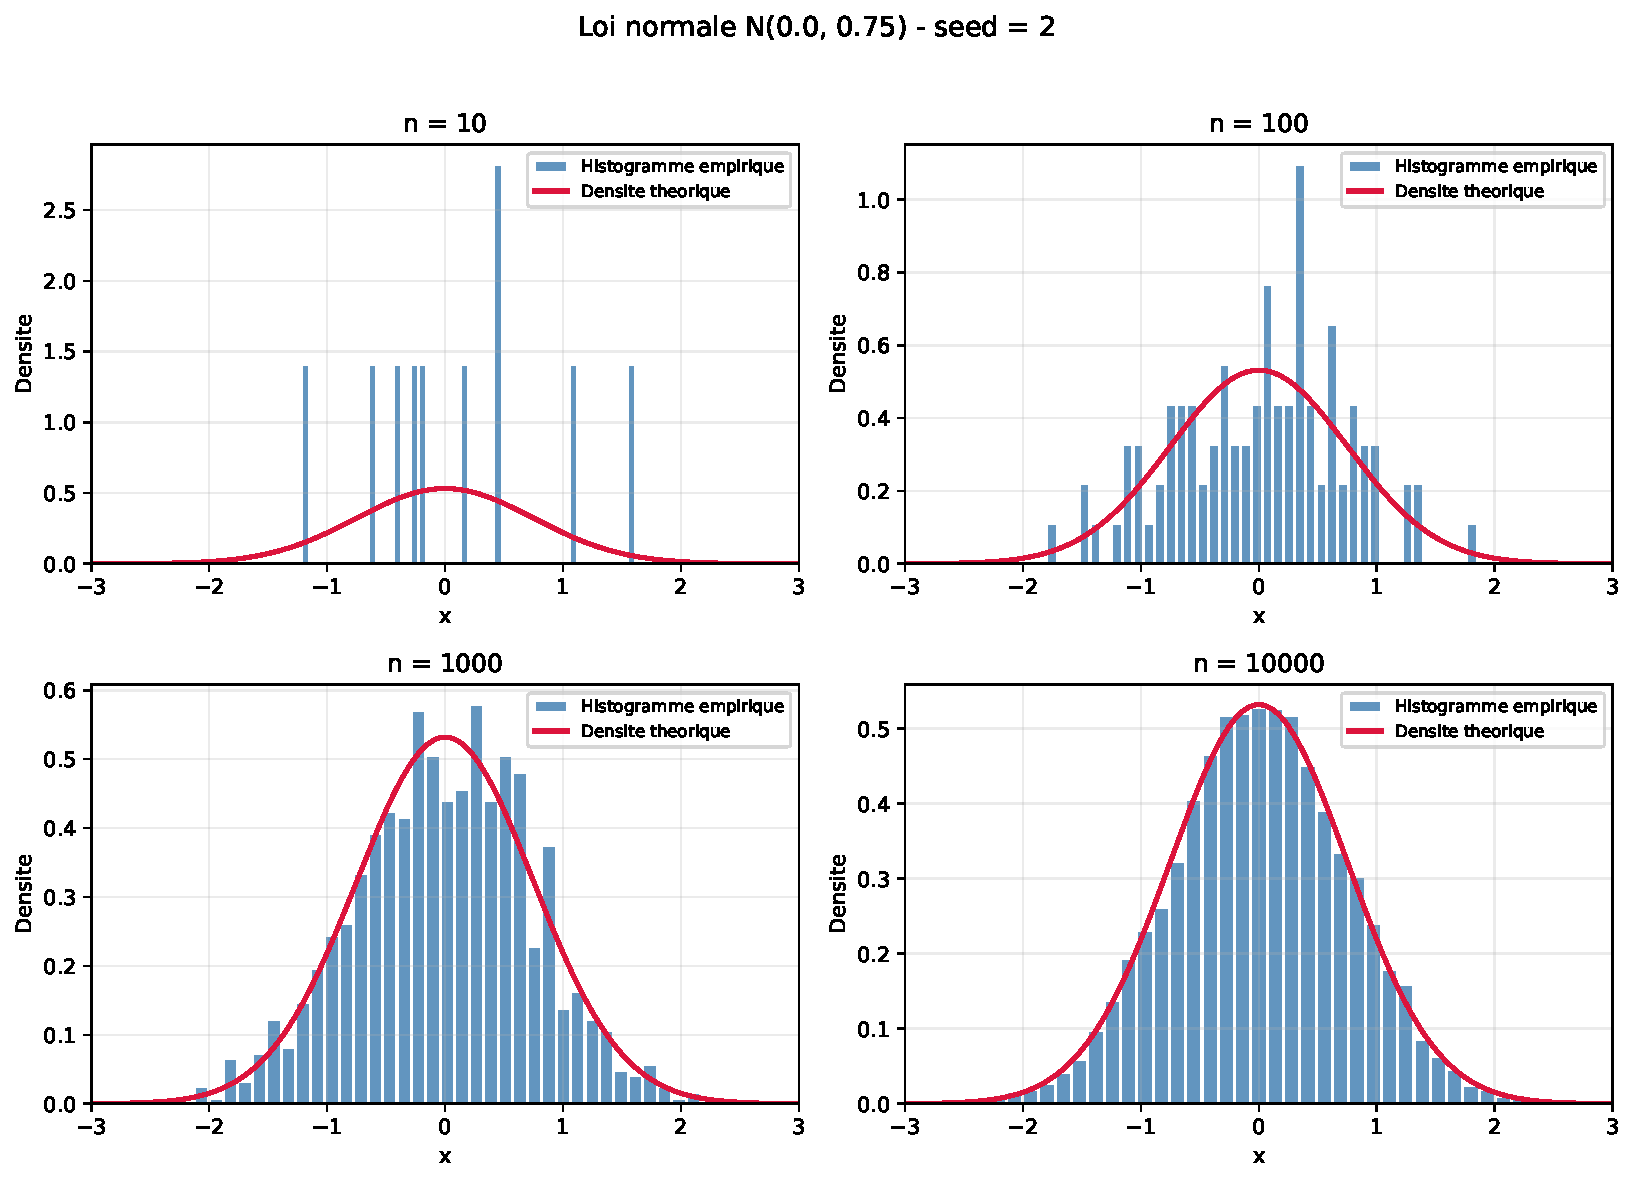
\includegraphics[width=0.9\linewidth]{hist_normale.pdf}
\caption{Histogrammes de la loi normale $\mathcal{N}(0, \sigma=0{,}75)$.}
\label{fig:hist-norm}
\end{figure}

\paragraph{Lecture.} On observe la c\'el\`ebre \og courbe en cloche\fg{} sym\'etrique
autour de $0$. \`A $n=10\,000$ l'histogramme \'epouse pr\'ecis\'ement la densit\'e
th\'eorique (rouge). La pr\'esence de quelques valeurs au-del\`a de $\pm 2{,}5$
(soit plus de $3$ \'ecarts-types) est compatible avec la probabilit\'e th\'eorique
$P(|X| > 3\sigma) \approx 0{,}27\%$, qui pr\'edit $\approx 27$ valeurs extr\^emes sur
$10\,000$ tirages -- proche de ce qu'on observe. C'est une bonne v\'erification
\og de coh\'erence\fg{} pour la m\'ethode Box--Muller.

% --------------------------------------------------------------------
% 8. Partie 4 : Analyse
% --------------------------------------------------------------------
\section{Analyse globale}
\label{sec:analyse}

\subsection{Convergence et loi des grands nombres}

La \emph{loi forte des grands nombres} affirme que pour $X_1, X_2, \ldots$
ind\'ependantes et de m\^eme loi, de moyenne $\mu$~:
\begin{equation*}
    \overline{X}_n = \frac{1}{n} \sum_{i=1}^{n} X_i \;\xrightarrow[n\to\infty]{\text{p.s.}}\; \mu.
\end{equation*}
La figure~\ref{fig:lln} illustre cette convergence pour quatre lois.

\begin{figure}[H]
\centering
\begin{subfigure}[t]{0.48\textwidth}
    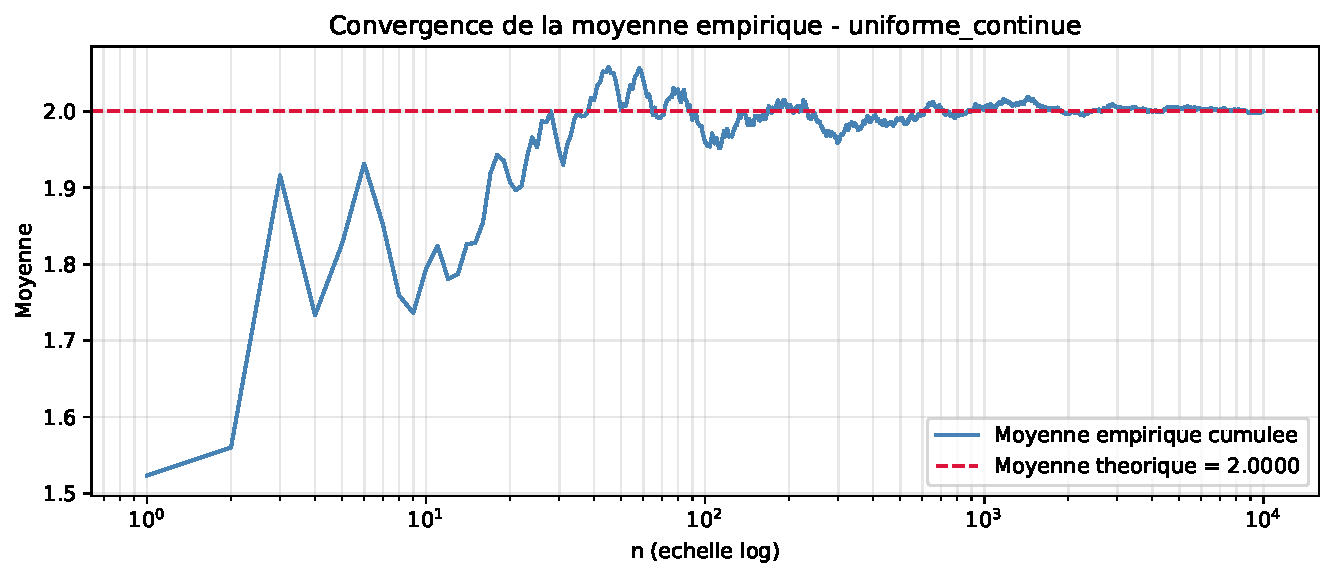
\includegraphics[width=\linewidth]{lln_uniforme_continue.pdf}
    \caption{Uniforme continue ($\mu = 2$).}
\end{subfigure}
\hfill
\begin{subfigure}[t]{0.48\textwidth}
    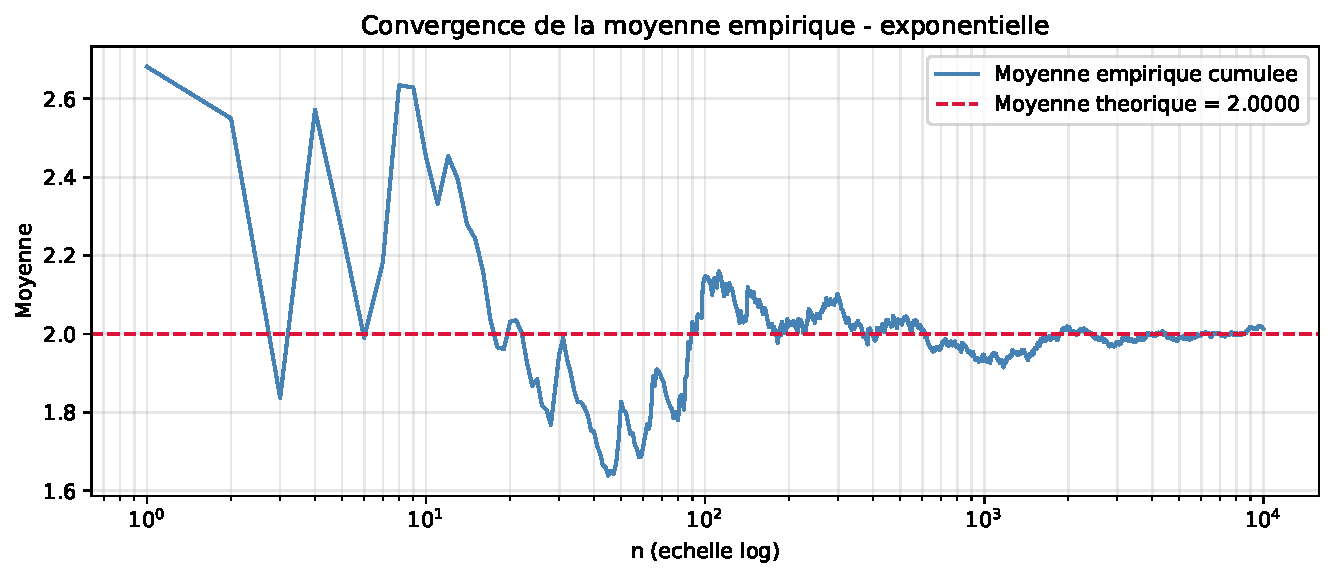
\includegraphics[width=\linewidth]{lln_exponentielle.pdf}
    \caption{Exponentielle ($\mu = 2$).}
\end{subfigure}\par\bigskip
\begin{subfigure}[t]{0.48\textwidth}
    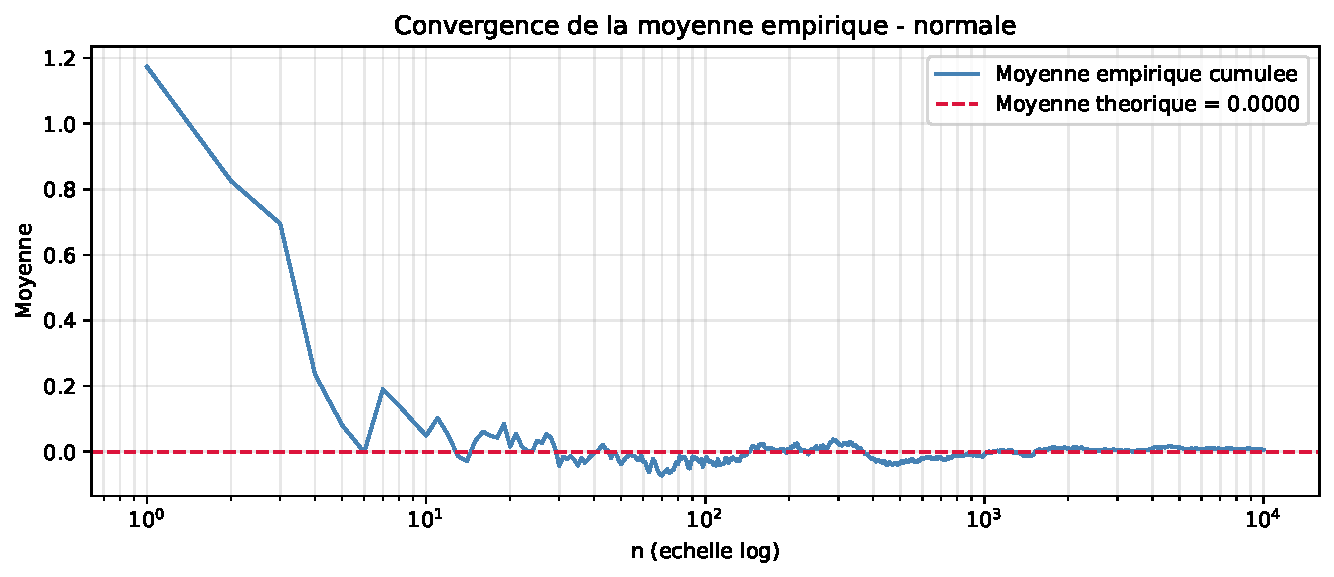
\includegraphics[width=\linewidth]{lln_normale.pdf}
    \caption{Normale ($\mu = 0$).}
\end{subfigure}
\hfill
\begin{subfigure}[t]{0.48\textwidth}
    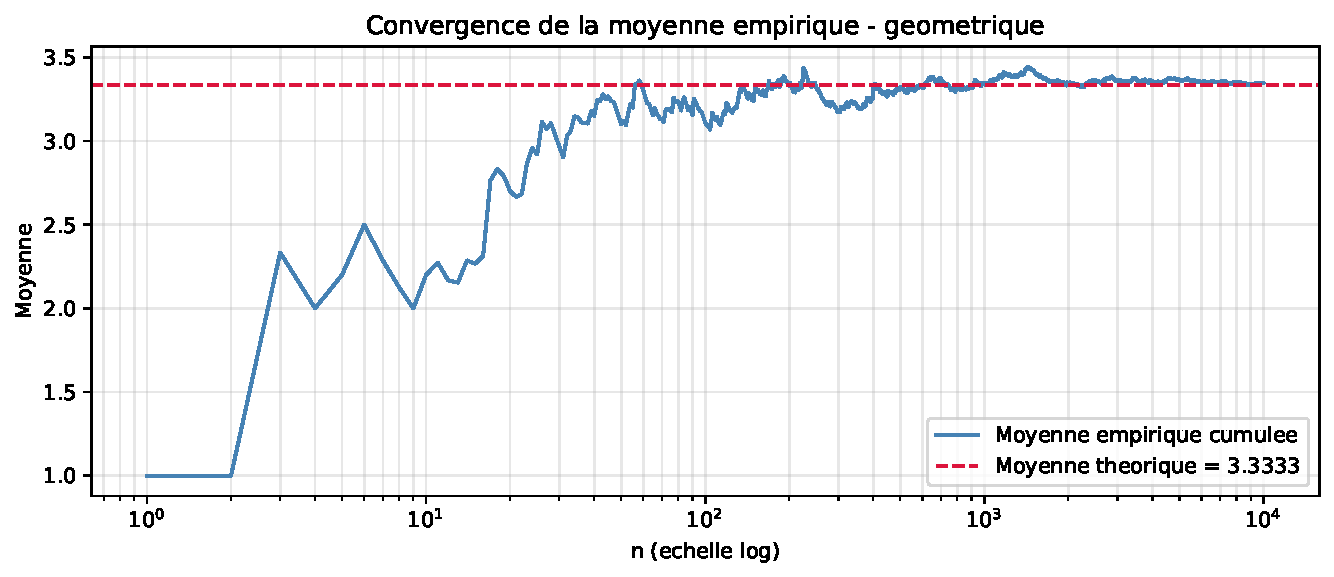
\includegraphics[width=\linewidth]{lln_geometrique.pdf}
    \caption{G\'eom\'etrique ($\mu = 1/p = 3{,}33$).}
\end{subfigure}
\caption{Convergence de la moyenne empirique cumul\'ee vers la moyenne th\'eorique (axe horizontal en \'echelle logarithmique).}
\label{fig:lln}
\end{figure}

\paragraph{Lecture.} Sur chacun des quatre panneaux on voit la courbe bleue
(moyenne cumul\'ee $\overline{X}_n$) osciller pour les petits $n$ puis se
\emph{stabiliser} autour de la ligne rouge (moyenne th\'eorique). Quelques
observations~:
\begin{itemize}
    \item La \emph{vitesse de convergence} est la m\^eme pour toutes (en
          $1/\sqrt{n}$) mais la \emph{magnitude des oscillations} d\'epend de la
          variance de la loi. L'exponentielle (variance $4$) oscille bien plus
          longtemps que la normale (variance $0{,}5625$) ou l'uniforme
          (variance $1/3$).
    \item La g\'eom\'etrique se stabilise un peu plus lentement \`a cause des
          \og queues longues\fg{}~: une tr\`es grande valeur (par ex.\ $X = 30$)
          peut faire monter la moyenne empirique \emph{brutalement}, ce qui se
          voit sur la courbe.
    \item Toutes les courbes convergent~; pour $n = 10\,000$ on est \`a
          quelques millicentaines de la valeur exacte. C'est la \emph{garantie}
          que les simulations sont quantitativement fiables si on prend
          suffisamment d'\'echantillons.
\end{itemize}

\subsection{Impact du nombre d'\'echantillons}

Le \emph{th\'eor\`eme central limite} pr\'edit que
$\sqrt{n}(\overline{X}_n - \mu) \to \mathcal{N}(0, \sigma^2)$~; en pratique,
l'erreur sur la moyenne empirique d\'ecro\^it en $\sigma/\sqrt{n}$. Pour
multiplier la pr\'ecision par 10, il faut donc multiplier $n$ par 100. C'est ce
qu'on voit aussi sur les histogrammes (sections pr\'ec\'edentes)~: \emph{seuls
les grands $n$ donnent des histogrammes lisses}.

\subsection{Impact de la graine}

La graine d\'etermine la suite obtenue mais ne change pas la loi cible. Avec
\texttt{seed = 2}, deux relances cons\'ecutives du code donnent \emph{exactement
les m\^emes valeurs} (voir fichiers \texttt{data/*.txt} fournis dans le rendu).
Pour estimer l'\emph{incertitude} d'une statistique on peut~:
\begin{itemize}
    \item soit relancer la simulation avec d'autres graines et calculer la
          dispersion des estimateurs~;
    \item soit s'appuyer sur la formule $\sigma/\sqrt{n}$ du TCL.
\end{itemize}

\subsection{Liens avec les syst\`emes informatiques}

Le tableau~\ref{tab:appli} r\'esume les usages les plus typiques des lois
\'etudi\'ees dans le monde des syst\`emes.

\begin{table}[H]
\centering
\caption{Liens entre les lois \'etudi\'ees et la mod\'elisation des syst\`emes informatiques.}
\label{tab:appli}
\begin{tabular}{ll}
\toprule
\textbf{Loi} & \textbf{Usage typique} \\
\midrule
Uniforme discr\`ete & S\'election al\'eatoire d'un serveur, d'un slot, d'une cl\'e de hachage. \\
Bernoulli           & Perte d'un paquet, succ\`es d'un essai. \\
G\'eom\'etrique     & Nombre de tentatives avant succ\`es (CSMA/CA, ALOHA, retry HTTP). \\
Poisson             & Nombre d'arriv\'ees de requ\^etes en un intervalle de temps (mod\`ele M/M/1). \\
Uniforme continue   & Temps de latence dans une fen\^etre $[a,b]$. \\
Exponentielle       & Temps inter-arriv\'ee, dur\'ee de service, MTBF. \\
Normale             & Bruit de mesure, latence centr\'ee, erreurs cumul\'ees (TCL). \\
\bottomrule
\end{tabular}
\end{table}

% --------------------------------------------------------------------
% 9. Conclusion
% --------------------------------------------------------------------
\section{Conclusion}

Ce TP a permis~:
\begin{enumerate}
    \item D'impl\'ementer et d'observer le comportement des g\'en\'erateurs
          congruentiels lin\'eaire et multiplicatif. Les exemples \og courts\fg{}
          ($m = 13$, $m = 16$) ont mis en \'evidence le cyclage~; le test des
          paires a r\'ev\'el\'e les structures cach\'ees de RANDU. Les bons
          g\'en\'erateurs (MINSTD, Numerical Recipes) ont des distributions
          uniformes correctes \`a notre \'echelle de $10^4$ tirages.
    \item De d\'eriver, depuis ces uniformes, les cinq lois demand\'ees pour le
          groupe~2 (uniforme discr\`ete $\{10,..,30\}$, uniforme continue
          $[1{,}0\,;\,3{,}0]$, normale $\mathcal{N}(0;\sigma=0{,}75)$, exponentielle
          de moyenne~2, g\'eom\'etrique $p=0{,}3$) gr\^ace \`a la \emph{m\'ethode de
          la transform\'ee inverse}, \`a \emph{Box--Muller}, et \`a l'\emph{algorithme
          de Knuth}.
    \item De v\'erifier exp\'erimentalement la convergence des estimateurs~:
          moyennes, \'ecarts-types et histogrammes empiriques approchent leurs
          valeurs th\'eoriques en $1/\sqrt{n}$, conform\'ement \`a la loi des
          grands nombres et au th\'eor\`eme central limite.
    \item De faire le lien entre ces outils probabilistes et la mod\'elisation
          concr\`ete des syst\`emes informatiques~: arriv\'ee de paquets, files
          d'attente, fiabilit\'e, MTBF, etc.
\end{enumerate}

Tous les codes, suites de valeurs et figures sont fournis dans l'archive
\texttt{TP\_Groupe2.zip}~; relancer \texttt{python3 src/main.py} reproduira
\emph{trait pour trait} les r\'esultats de ce rapport.

\bigskip
\hrule
\bigskip
\paragraph{R\'ef\'erences principales utilis\'ees~:}
\begin{itemize}
    \item Knuth, D.E.\ \emph{The Art of Computer Programming, Vol.~2}.
    \item Park, S.K.\ \& Miller, K.W.\ (1988). \emph{Random number generators: good ones are hard to find.}
    \item L'Ecuyer, P.\ \emph{Tables of Linear Congruential Generators of Different Sizes.}
    \item Cours RCP103 -- Pedro Braconnot Velloso, CNAM Paris.
\end{itemize}

\end{document}
